\documentclass{report}

\input{~/dev/latex/template/preamble.tex}
\input{~/dev/latex/template/macros.tex}

\title{\Huge{}}
\author{\huge{Nathan Warner}}
\date{\huge{}}
\pagestyle{fancy}
\fancyhf{}
\rhead{}
\fancyhead[R]{\itshape Warner} % Right header: Last Name
\fancyhead[L]{\itshape\leftmark}  % Right header: Section Name
\cfoot{\thepage}
\renewcommand{\headrulewidth}{0pt} % Remove the header line

% Change the title
\hypersetup{
	pdftitle={Math 2}
}


\begin{document}
    % \maketitle
        \begin{titlepage}
       \begin{center}
           \vspace*{1cm}
    
           \textbf{Comprehensive Compendium:} \\
            Calculus II
    
           \vspace{0.5cm}
            
                
           \vspace{1.5cm}
    
           \textbf{Nathan Warner}
    
           \vfill
                
                
           \vspace{0.8cm}
         
           
\includegraphics[width=0.4\textwidth]{~/niu/seal.png}
                
           Computer Science \\
           Northern Illinois University\\
           August 28,2023 \\
           United States\\
           
                
       \end{center}
    \end{titlepage}
    \tableofcontents
    \pagebreak \bigbreak \noindent
    \unsect{Calculus II}
    \bigbreak \noindent 

    \bigbreak \noindent 
    \subsection{Chapter 1 Definitions and Theorems}
    \bigbreak \noindent 
    \begin{itemize}
        \item \textbf{Mean Value Theorem For Integrals}: If  $f(x)$ is continuous over an interval  [a,b], then there is at least one point  $c\in[a,b]$ such that 
            \begin{align*}
                f(c) = \frac{1}{b-a}\int f(x)\ dx
            .\end{align*}
        \item \textbf{Integrals resulting in inverse trig functions}
            \begin{enumerate}
                \item \begin{align*}
                        \int \frac{dx}{\sqrt{a^{2}-x^{2}}} = \sin^{-1}{\frac{x}{\abs{a}}} + C
                    .\end{align*}
                \item \begin{align*}
                        \int \frac{dx}{a^{2}+x^{2}} = \frac{1}{a}\tan^{-1}{\frac{x}{a}} + C
                    .\end{align*}
                \item \begin{align*}
                        \int \frac{dx}{x\sqrt{x^{2}-a^{2}}} = \frac{1}{\abs{a}}\sec^{-1}{\frac{\abs{x}}{a}} + C
                    .\end{align*}
            \end{enumerate}
    \end{itemize}

    % \pagebreak \bigbreak \noindent 
    % \subsection{Chapter 2 Key Terms / Ideas}
    % \bigbreak \noindent 
    % \begin{itemize}
    %     \item \textbf{Finding limits of integration for region between two functions}: Usually, we want our limits of integration to be the points where the functions intersect
    %     \item A \textbf{"complex region"} between curves usually refers to an area that is not easily described by a single, continuous function over the interval of interest.
    %     \item \textbf{compound regions} are regions bounded by the graphs of functions that cross one another
    %     \item \textbf{Cross-section:} The intersection of a plane and a solid object.
    %     \item a \textbf{cylinder} is a three-dimensional shape that has two parallel, congruent bases connected by a curved surface. The bases are usually circles, but they can be other shapes as well
    %     \item The line segment connecting the centers of the two bases is called the \textbf{"axis" of the cylinder.}
    %     \item \textbf{Slicing method:} A method of calculating the volume of a solid that involves cutting the solid into pieces, estimating the volume of each piece, then adding these estimates to arrive at an estimate of the total volume; as the number of slices goes to infinity, this estimate becomes an integral that gives the exact value of the volume.
    %     \begin{enumerate}
    %         \item Examine the solid and determine the shape of a cross-section of the solid. It is often helpful to draw a picture if one is not provided.
    %         \item Determine a formula for the area of the cross-section.
    %         \item Integrate the area formula over the appropriate interval to get the volume.
    %     \end{enumerate}
    %     \item \textbf{Solid of revolution:} A solid generated by revolving a region in a plane around a line in that plane.
    %     \item \textbf{Disk method:} A special case of the slicing method used with solids of revolution when the slices are disks.
    %     \item A \textbf{Washer (Annuli)} is a disk with holes in the center.
    %     \item \textbf{Washer method:} A special case of the slicing method used with solids of revolution when the slices are washers.
    %     \item \textbf{Method of cylindrical shells:} A method of calculating the volume of a solid of revolution by dividing the solid into nested cylindrical shells; this method is different from the methods of disks or washers in that we integrate with respect to the opposite variable.
    %     % \item A \textbf{cylinder} is defined as any solid that can be generated by translating a plane region along a line perpendicular to the region, called the \textbf{axis of the cylinder}.
    %      \item \textbf{Arc length:} The arc length of a curve can be thought of as the distance a person would travel along the path of the curve.
    %     \item \textbf{Surface area:} The surface area of a solid is the total area of the outer layer of the object; for objects such as cubes or bricks, the surface area of the object is the sum of the areas of all of its faces.
    %     % \item \textbf{Catenary:} A curve in the shape of the function \(y = a \cosh(x/a)\) is a catenary; a cable of uniform density suspended between two supports assumes the shape of a catenary.
    %     % \item \textbf{Center of mass:} The point at which the total mass of the system could be concentrated without changing the moment.
    %     % \item \textbf{Centroid:} The centroid of a region is the geometric center of the region; laminas are often represented by regions in the plane; if the lamina has a constant density, the center of mass of the lamina depends only on the shape of the corresponding planar region; in this case, the center of mass of the lamina corresponds to the centroid of the representative region.
    %     % \item \textbf{Density function:} A density function describes how mass is distributed throughout an object; it can be a linear density, expressed in terms of mass per unit length; an area density, expressed in terms of mass per unit area; or a volume density, expressed in terms of mass per unit volume; weight-density is also used to describe weight (rather than mass) per unit volume.
    %     % \item \textbf{Doubling time:} If a quantity grows exponentially, the doubling time is the amount of time it takes the quantity to double, and is given by \(\frac{\ln 2}{k}\).
    %     % \item \textbf{Exponential decay:} Systems that exhibit exponential decay follow a model of the form \(y = y_0 e^{-kt}\).
    %     % \item \textbf{Exponential growth:} Systems that exhibit exponential growth follow a model of the form \(y = y_0 e^{kt}\).
    %     % \item \textbf{Frustum:} A portion of a cone; a frustum is constructed by cutting the cone with a plane parallel to the base.
    %     % \item \textbf{Half-life:} If a quantity decays exponentially, the half-life is the amount of time it takes the quantity to be reduced by half. It is given by \(\frac{\ln 2}{k}\).
    %     % \item \textbf{Hooke's Law:} This law states that the force required to compress (or elongate) a spring is proportional to the distance the spring has been compressed (or stretched) from equilibrium; in other words, \(F = kx\), where \(k\) is a constant.
    %     % \item \textbf{Hydrostatic pressure:} The pressure exerted by water on a submerged object.
    %     % \item \textbf{Lamina:} A thin sheet of material; laminas are thin enough that, for mathematical purposes, they can be treated as if they are two-dimensional.
    %     % \item \textbf{Moment:} If \(n\) masses are arranged on a number line, the moment of the system with respect to the origin is given by \(M = \sum_{i=1}^{n} m_i x_i\); if, instead, we consider a region in the plane, bounded above by a function \(f(x)\) over an interval \([a, b]\), then the moments of the region with respect to the \(x\)- and \(y\)-axes are given by \(M_x = \rho \int_{a}^{b} \frac{[f(x)]^2}{2} dx\) and \(M_y = \rho \int_{a}^{b} x f(x) dx\), respectively.
    %     % \item \textbf{Symmetry principle:} The symmetry principle states that if a region \(R\) is symmetric about a line \(l\), then the centroid of \(R\) lies on \(l\).
    %     % \item \textbf{Theorem of Pappus for volume:} This theorem states that the volume of a solid of revolution formed by revolving a region around an external axis is equal to the area of the region multiplied by the distance traveled by the centroid of the region.
    %     % \item \textbf{Work:} The amount of energy it takes to move an object; in physics, when a force is constant, work is expressed as the product of force and distance.
    % \end{itemize}

    \pagebreak \bigbreak \noindent 
    \subsection{Chapter 2 Definitions and Theorems}
    \bigbreak \noindent 
    \begin{itemize}

        \item \textbf{Area between two curves, integrating on the x-axis}
            \begin{align}
                A = \int_{a}^{b} [f(x) - g(x)] \, dx
            \end{align}
            Where $f(x) \geq g(x)$
            \begin{align*}
                A = \int_{a}^{b}\ [g(x) - f(x)]\ dx
            .\end{align*}
            for $g(x) \geq f(x)$

        \item \textbf{Area between two curves, integrating on the y-axis}
            \begin{align}
                A = \int_{c}^{d} [u(y) - v(y)] \, dy
            \end{align}

        \item \textbf{Areas of compound regions}
            \begin{align*}
                \int_{a}^{b}\ \abs{f(x)-g(x)}\ dx 
            .\end{align*}
        \item \textbf{Area of complex regions}
            \begin{align*}
                \int_{a}^{b}\ f(x)\ dx + \int_{b}^{c}\ g(x)\ dx
            .\end{align*}
        \item \textbf{Slicing Method}
            \begin{align*}
                V(s) = \summation{n}{i=1}\ A(x_{i}^{*})\ \Delta x  = \int_{a}^{b}\ A(x)\ dx
            .\end{align*}
        \item \textbf{Disk Method along the x-axis}
            \begin{align}
                V = \int_{a}^{b} \pi [f(x)]^2 \, dx
            \end{align}

        \item \textbf{Disk Method along the y-axis}
            \begin{align}
                V = \int_{c}^{d} \pi [g(y)]^2 \, dy
            \end{align}

        \item \textbf{Washer Method along the x-axis}
            \begin{align}
                V = \int_{a}^{b} \pi [(f(x))^2 - (g(x))^2] \, dx
            \end{align}

        \item \textbf{Washer Method along the y-axis}
            \begin{align}
                V = \int_{c}^{d} \pi [(u(y))^2 - (v(y))^2] \, dy
            \end{align}

        \item \textbf{Radius if revolved around other line (Washer Method)}
            \begin{align*}
                If:\ x=-k\\
                Then:\ r = Function + k
            .\end{align*}
            \begin{align*}
                If:\ x=k\\
                Then:\ r = k - Function
            .\end{align*}

        \item \textbf{Method of Cylindrical Shells (x-axis)}
            \begin{align}
                V = \int_{a}^{b} 2\pi x f(x) \, dx
            \end{align}

        \item \textbf{Method of Cylindrical Shells (y-axis)}
            \begin{align}
                V = \int_{c}^{d} 2\pi y g(y) \, dy
            \end{align}

        \item \textbf{Region revolved around other line (method of cylindrical shells):}
            \begin{align*}
                If:\ x=-k \\
                Then:\ V = \int_{a}^{b}\ 2\pi (x+k)(f(x))\ dx
            .\end{align*}
            \begin{align*}
                If:\ x=k \\
                Then:\ V = \int_{a}^{b}\ 2\pi (k-x)(f(x))\ dx
            .\end{align*}
        \item \textbf{A Region of Revolution Bounded by the Graphs of Two Functions (method cylindrical shells)}
            \begin{align*}
                V = \int_{a}^{b}\ 2\pi x\left[f(x)-g(x)\right]\ dx
            .\end{align*}

        \item \textbf{Arc Length of a Function of x}
            \begin{align}
                \text{Arc Length} = \int_{a}^{b} \sqrt{1 + [f'(x)]^2} \, dx
            \end{align}

        \item \textbf{Arc Length of a Function of y}
            \begin{align}
                \text{Arc Length} = \int_{c}^{d} \sqrt{1 + [g'(y)]^2} \, dy
            \end{align}

        \item \textbf{Surface Area of a Function of x (Around x)}
            \begin{align}
                \text{Surface Area} = \int_{a}^{b} 2\pi f(x) \sqrt{1 + [f'(x)]^2} \, dx
            \end{align}

        \item \textbf{Surface Area of a Function of x (Around y)}
            \begin{align}
                \text{Surface Area} = \int_{a}^{b} 2\pi \sqrt{1 + [f'(x)]^2} \, dx \\
                \text{Or: } \int_{a}^{b}\ 2\pi u(y)\sqrt{1+(u^{\prime}(y))^{2}}\ dy
            \end{align}

        \item \textbf{Natural logarithm function}
            \begin{align}
                \ln x = \int_{1}^{x} \frac{1}{t} \, dt\
            \end{align}

        \item \textbf{Exponential function}
            \begin{align}
                y = e^x, \quad \ln y = \ln(e^x) = x\
            \end{align}

        \item  \textbf{Logarithm Differentiation}
            \begin{align*}
                f^{\prime}(x) = f(x) \cdot \frac{d}{dx}\ln{\left(f^{\prime}(x)\right)}
            .\end{align*}
            \textbf{Note:} Use properties of logs before you differentiate whats inside the logarithm

            % \item \textbf{Mass of a one-dimensional object}
            % \begin{align}
            %     m = \int_{a}^{b} \rho(x) \, dx
            % \end{align}
            %
            % \item \textbf{Mass of a circular object}
            % \begin{align}
            %     m = \int_{0}^{r} 2\pi x \rho(x) \, dx
            % \end{align}
            %
            % \item \textbf{Work done on an object}
            % \begin{align}
            %     W = \int_{a}^{b} F(x) \, dx
            % \end{align}
            %
            % \item \textbf{Hydrostatic force on a plate}
            % \begin{align}
            %     F = \int_{a}^{b} \rho w(x) s(x) \, dx
            % \end{align}
            %
            % \item \textbf{Mass of a lamina}
            % \begin{align}
            %     m = \rho \int_{a}^{b} f(x) \, dx
            % \end{align}
            %
            % \item \textbf{Moments of a lamina}
            % \begin{align}
            %     M_x = \rho \int_{a}^{b} \frac{[f(x)]^2}{2} \, dx, \quad M_y = \rho \int_{a}^{b} x f(x) \, dx
            % \end{align}
            %
            % \item \textbf{Center of mass of a lamina}
            % \begin{align}
            %     \bar{x} = \frac{M_y}{m},\ \ \text{and}\ \  \bar{y} = \frac{M_x}{m}
            % \end{align}

    \end{itemize}


    % \pagebreak \bigbreak \noindent 
    % \subsection{Chapter 3 Key Terms}
    % \bigbreak \noindent 
    % \begin{itemize}
    %     \item \textbf{integration by parts}: a technique of integration that allows the exchange of one integral for another using the formula 
    %     \item \textbf{integration table}: a table that lists integration formulas.
    %     \item \textbf{power reduction formula}: a rule that allows an integral of a power of a trigonometric function to be exchanged for an integral involving a lower power.
    %     \item \textbf{trigonometric integral}: an integral involving powers and products of trigonometric functions.
    %     \item \textbf{trigonometric substitution}: an integration technique that converts an algebraic integral containing expressions of the form \( \sqrt{a^2 - x^2} \), \( \sqrt{a^2 + x^2} \), or \( \sqrt{x^2 - a^2} \) into a trigonometric integral.
    %     \item \textbf{partial fraction decomposition}: a technique used to break down a rational function into the sum of simple rational functions.
    %     \item \textbf{improper integral}: an integral over an infinite interval or an integral of a function containing an infinite discontinuity on the interval; an improper integral is defined in terms of a limit. The improper integral converges if this limit is a finite real number; otherwise, the improper integral diverges.
    %      % \item \textbf{absolute error}: if \( B \) is an estimate of some quantity having an actual value of \( A \), then the absolute error is given by \( |A-B| \).
    %     % \item \textbf{computer algebra system (CAS)}: technology used to perform many mathematical tasks, including integration.
    %     % \item \textbf{midpoint rule}: a rule that uses a Riemann sum of the form 
    %     % \item \textbf{numerical integration}: the variety of numerical methods used to estimate the value of a definite integral, including the midpoint rule, trapezoidal rule, and Simpson’s rule.
    %     % \item \textbf{relative error}: error as a percentage of the absolute value, given by 
    %     % \item \textbf{Simpson’s rule}: a rule that approximates \( \int_{a}^{b} f(x) \, dx \) using the integrals of a piecewise quadratic function. The approximation \( S_n \) to \( \int_{a}^{b} f(x) \, dx \) is given by 
    %     % \item \textbf{trapezoidal rule}: a rule that approximates \( \int_{a}^{b} f(x) \, dx \) using trapezoids.
    % \end{itemize}
    %
    \pagebreak \bigbreak \noindent 
    \subsection{Chapter 3 Definitions and Theorems}
    \bigbreak \noindent 
    \begin{itemize}
        \item \textbf{Integration by parts formula} 
            \begin{align*}
                \int u \, dv &= uv - \int v \, du 
            .\end{align*}
        \item \textbf{Integration by parts for definite integral}
            \begin{align*}
                \int_{a}^{b} u \, dv &= uv\big|_{a}^{b} - \int_{a}^{b} v \, du
            \end{align*}
        \item \textbf{To integrate products involving  sin(ax), sin(bx), cos(ax), and  cos(bx), use the substitutions:}
            \begin{itemize}
                \item \textbf{Sine Products}
                    \begin{align*}
                        \sin(ax) \sin(bx) &= \frac{1}{2} \cos((a-b)x) - \frac{1}{2} \cos((a+b)x)
                    \end{align*}

                \item \textbf{Sine and Cosine Products}
                    \begin{align*}
                        \sin(ax) \cos(bx) &= \frac{1}{2} \sin((a-b)x) + \frac{1}{2} \sin((a+b)x)
                    \end{align*}

                \item \textbf{Cosine Products}
                    \begin{align*}
                        \cos(ax) \cos(bx) &= \frac{1}{2} \cos((a-b)x) + \frac{1}{2} \cos((a+b)x)
                    \end{align*}

                \item \textbf{Power Reduction Formula (sine)}
                    \begin{align*}
                        &\int \sin^{n}{x}\ dx = -\frac{1}{n}\sin^{n-1}{x}\cos{x} + \frac{n-1}{n}\int \sin^{n-2}{x}\ dx \\
                        &\int_{0}^{\frac{\pi}{2}}\ \sin^{n}{x}\ dx = \frac{n-1}{n}\int_{0}^{\frac{\pi}{2}}\ \sin^{n-2}{x}\ dx
                    .\end{align*}
                \item \textbf{Power Reduction Formula (cosine)}
                    \begin{align*}
                        &\int \cos^{n}{x}\ dx = \frac{1}{n}\cos^{n-1}{x}\sin{x} + \frac{n-1}{n}\int \cos^{n-2}{x}\ dx \\
                        &\int_{0}^{\frac{\pi}{2}}\ \cos^{n}{x}\ dx = \frac{n-1}{n}\int_{0}^{\frac{\pi}{2}}\ \cos^{n-2}{x}\ dx
                    .\end{align*}
                \item \textbf{Power Reduction Formula (secant)}
                    \begin{align*}
                        \int \sec^{n}{x}\ dx &= \frac{1}{n-1}\sec^{n-1}{x}\sin{x}+\frac{n-2}{n-1}\int \sec^{n-2}{x}\ dx \\
                        \int \sec^{n}{x}\ dx &= \frac{1}{n-1}\sec^{n-2}{x}\tan{x}+\frac{n-2}{n-1}\int \sec^{n-2}{x}\ dx
                    \end{align*}

                \item \textbf{Power Reduction Formula (tangent)}
                    \begin{align*}
                        \int \tan^n x \, dx &= \frac{1}{n-1} \tan^{n-1}x - \int \tan^{n-2}x \, dx
                    \end{align*}
            \end{itemize}
        \item \textbf{Trigonometric Substitution}
            \begin{itemize}
                \item $\sqrt{a^{2} - x^{2}}$ use $x =a\sin{\theta }$ with domain restriction $\bigg[-\frac{\pi}{2},\frac{\pi}{2}\bigg] $
                \item $\sqrt{a^{2} + x^{2}}$ use $x=a\tan{\theta}$ with domain restriction $\left(-\frac{\pi}{2}, \frac{\pi}{2}\right)$
                \item $\sqrt{x^{2} - a^{2}}$ use $x =a\sec{\theta}$ with domain restriction $\bigg[0,\frac{\pi}{2}\bigg) \cup \bigg[\pi,\frac{3\pi}{2}\bigg)$ 
            \end{itemize}

        \item \textbf{Steps for fraction decomposition}
            \begin{enumerate}
                \item Ensure $deg(Q) < deg(P)$, if not, long divide
                \item Factor denominator
                \item Split up fraction into factors
                \item Multiply through to clear denominator
                \item Group terms and equalize
                \item Solve for constants
                \item Plug constants into split up fraction
                \item Compute integral
            \end{enumerate}

        \item \textbf{Solving for constants}
            Either:
            \begin{itemize}
                \item Plug in values (often the roots)
                \item Equalize 
            \end{itemize}
        \item \textbf{Cases for partial fractions}
            \begin{itemize}
                \item Non repeated linear factors
                \item Repeated linear factors
                \item Nonfactorable quadratic factors
            \end{itemize}
        \item \textbf{Midpoint rule}
            \begin{align*}
                M_{n} = \summation{n}{i=1}\ f(m_{i})\ \Delta x 
            .\end{align*}
        \item \textbf{Absolute error}
            \begin{align*}
                err = \bigg|\text{Actual} - \text{Estimated}\bigg|
            .\end{align*}
        \item \textbf{Relative error}
            \begin{align*}
                err = \bigg|\frac{\text{Actual} - \text{Estimated}}{\text{Actual}}\bigg| \cdot 100\%
            .\end{align*}
        \item \textbf{Error upper bound for midpoint rule}
            \begin{align*}
                E_{M} \leq \frac{M(b-a)^3}{24n^2}
            \end{align*}
            Where $M$ is the maximum value of the second derivative
        \item \textbf{Trapezoidal rule}
            \begin{align*}
                T_n \frac{1}{2} \Delta x \left( f(x_0) + 2f(x_1) + 2f(x_2) + \cdots + 2f(x_{n-1}) + f(x_n) \right)
            \end{align*}
        \item \textbf{Error upper bound for trapezoidal rule}
            \begin{align*}
                E_{T} \leq \frac{M(b-a)^3}{12n^2}
            \end{align*}
            Where $M$ is the maximum value of the second derivative
        \item \textbf{Simpson’s rule}
            \begin{align*}
                S_n = \frac{\Delta x}{3} \left( f(x_0) + 4f(x_1) + 2f(x_2) + 4f(x_3) + 2f(x_4) + 4f(x_5) + \cdots + 2f(x_{n-2}) + 4f(x_{n-1}) + f(x_n) \right)
            \end{align*}
        \item \textbf{Error upper bound for Simpson’s rule}
            \begin{align*}
                E_{S} \leq \frac{M(b-a)^5}{180n^4}
            \end{align*}
            Where $M$ is the maximum value of the fourth derivative
        \item \textbf{Finding $n$ with error bound functions}
            \begin{enumerate}
                \item Find $f^{\prime\prime}(x)$
                \item Find maximum values of $f^{\prime\prime}(x)$ in the interval
                \item Plug into error bound function 
                \item Set value $\leq$ desired accuracy (ex: 0.01)
                \item Solve: 
                \item If we were to truncate, we would use the ceil function $\ceil*{n}$ DO NOT FLOOR
            \end{enumerate}
        \item \textbf{Improper integrals (Infinite interval)}
            \begin{itemize}
                \item $\int_{a}^{+\infty}\ f(x)\ dx  = \lim\limits_{t \to +\infty}{\int_{a}^{t}\ f(x)\ dx}$  
                \item $\int_{-\infty}^{b}\ f(x)\ dx = \lim\limits_{t \to -\infty}{\int_{t}^{b}\ f(x)\ dx}$ 
                \item $\int_{-\infty}^{+\infty}\ f(x)\ dx = \int_{-\infty}^{0}\ f(x)\ dx + \int_{0}^{+\infty}\ f(x)\ dx$
            \end{itemize}
        \item \textbf{Improper integral (discontinuous)}
            \begin{itemize}
                \item Let $f(x)$ be continuous on $[a,b)$, then;
                    \begin{align*}
                        \int_{a}^{b}\ f(x)\ dx = \lim\limits_{t \to b^{-}}{\int_{a}^{t}\ f(x)\ dx}\
                    .\end{align*}
                \item Let $f(x)$ be continuous on $(a,b]$, then;
                    \begin{align*}
                        \int_{a}^{b}\ f(x)\ dx = \lim\limits_{t \to b^{+}}{\int_{t}^{b}\ f(x)\ dx}\
                    .\end{align*}
                    In each case, if the limit exists, then the improper integral is said to converge. If the limit does not exist, then the improper integral is said to diverge.
                \item Let $f(x)$ be continuous on $[a,b]$ except at a point $c \in (a,b)$, then;
                    \begin{align*}
                        \int_{a}^{b}\ f(x)\ dx = \int_{a}^{c}\ f(x)\ dx  +\int_{c}^{b}\ f(x)\ dx
                    .\end{align*}
                    If either integral diverges, then $\int_{a}^{b}\ f(x)\ dx $ diverges
            \end{itemize}
        \item \textbf{Comparison theorem}
            Let $f(x)$ and $g(x)$ be continuous over $[a,+\infty)$. Assume that $0 \leq f(x) \leq g(x)$ for $x \geq a$.
            \begin{itemize}
                \item If $\int_a^{+\infty} f(x) \, dx = \lim_{t \to +\infty} \int_a^t f(x) \, dx = +\infty$,  \\
                    then $\int_a^{+\infty} g(x) \, dx = \lim_{t \to +\infty} \int_a^t g(x) \, dx = +\infty$.
                \item If $\int_a^{+\infty} g(x) \, dx = \lim_{t \to +\infty} \int_a^t g(x) \, dx = L$, where $L$ is a real number,  \\
                    then $\int_a^{+\infty} f(x) \, dx = \lim_{t \to +\infty} \int_a^t f(x) \, dx = M$ for some real number $M \leq L$.
            \end{itemize}
            \pagebreak \bigbreak \noindent 
        \item \textbf{P-integrals}
            \begin{itemize}
                \item $\int_{0}^{+\infty} \frac{1}{x^{p}}\ dx =  
                    \begin{cases}
                        \frac{1}{p-1} & \text{if } p>1 \\
                        +\infty & \text{if } p \leq 1
                    \end{cases}$
                \item $\int_{0}^{1} \frac{1}{x^p}\ dx =    
                    \begin{cases}
                        \frac{1}{1-p} & \text{if } p<1 \\
                        +\infty & \text{if } p \geq 1
                    \end{cases}$
                \item $\int_{a}^{+\infty} \frac{1}{x^{p}}\ dx =  
                    \begin{cases}
                        \frac{a^{1-p}}{p-1} & \text{if } p>1 \\
                        +\infty & \text{if } p \leq 1
                    \end{cases}$
                \item $\int_{0}^{a} \frac{1}{x^p}\ dx =    
                    \begin{cases}
                        \frac{a^{1-p}}{1-p} & \text{if } p<1 \\
                        +\infty & \text{if } p \geq 1
                    \end{cases}$
            \end{itemize}
        \item \textbf{Bypass L'Hospital's Rule}
            \begin{align*}
                \ln{(\ln{(x)})},\ \ln{(x)},\ \cdots\ x^{\frac{1}{100}},\ x^{\frac{1}{3}},\ \sqrt{x},\ 1,\ x^{2},\ x^{3},\ \cdots\ e^{x},\ e^{2x},\ e^{3x},\ \cdots,\ e^{x^{2}},\ \cdots\ e^{e^{x}}
            .\end{align*}
            Essentially what it means is things on the right grow faster than things on the left. Thus, if we have say:
            \begin{align*}
                \lim\limits_{x \to \infty}{\frac{x^{2}}{e^{2x}}} 
            .\end{align*}
            We can be sure that it is zero. Because this is $x^{2}\cdot e^{-2x}$. If we take  $ \lim\limits_{x \to \infty}{x^{2}e^{-2x}}$, we get $\infty \cdot 0$. As we see by the sequence $e^{-2x}$ overrules $x^{2}$ and we can say the limit is zero.
            % \item \textbf{something to consider for limits}: Suppose we have $f:\ A \rightarrow B:\ x \mapsto f(x)$. It would not be meaninful to consider some $ \lim\limits_{x \to b+n}{f(x)}$ for $n>0 $. Thus we shall conclude that the limit is undefined. For example, the domain of arcsine is $[-1,1]$, thus any $\lim\limits_{x \to a}{f(x)}$ for $(-\infty,-1)\cup (1,\infty)$ would be undefined
        \item \textbf{Consideration for Limits}: Let \(f: A \rightarrow B\) be a function defined by \(x \mapsto f(x)\). If a point \(c\) lies outside the domain \(A\), then the expression \(\lim\limits_{x \to c} f(x)\) is not meaningful, and we classify this limit as undefined. For instance, the function arcsine has a domain of \([-1,1]\). Therefore, limits like \(\lim\limits_{x \to a} \sin^{-1}(x)\) where \(a \notin [-1,1]\) are undefined.
        \item \textbf{Why does}
            \begin{align*}
            &\lim\limits_{x \to 2}{\tan^{-1}{\frac{1}{x-2}}} 
        .\end{align*}
        \begin{minipage}[]{0.47\textwidth}
            \begin{align*}
                &=\lim\limits_{x \to 2^{-}}{\tan^{-1}{\frac{1}{x-2}}} \\
                &= \lim\limits_{x \to -\infty}{\tan^{-1}{x}} \\
                &= -\pi/2
            .\end{align*}
        \end{minipage}
        \begin{minipage}[]{0.47\textwidth}
            \begin{align*}
                &=\lim\limits_{x \to 2^{+}}{\tan^{-1}{\frac{1}{x-2}}} \\
                &=\lim\limits_{x \to +\infty}{\tan^{-1}{x}} \\
                &=\frac{\pi}{2}
            .\end{align*}
        \end{minipage}
\end{itemize}

% \pagebreak \bigbreak \noindent 
% \subsection{Chapter 5 Key Terms}
% \bigbreak \noindent 
% \begin{itemize}
% 
% \item Alternating series: 
% \[
% \text{A series of the form } \sum_{n=1}^{\infty} (-1)^{n+1} b_n \text{ or } \sum_{n=1}^{\infty} (-1)^n b_n, \text{ where } b_n \geq 0, \text{ is called an alternating series.}
% \]
% 
% \item Alternating series test: 
% \[
% \text{For an alternating series of either form, if } b_{n+1} \leq b_n \text{ for all integers } n \geq 1 \text{ and } b_n \to 0, \text{ then an alternating series converges.}
% \]
% 
% \item Arithmetic sequence: 
% \[
% \text{A sequence in which the difference between every pair of consecutive terms is the same is called an arithmetic sequence.}
% \]
% 
% \item Bounded above: 
% \[
% \text{A sequence } \{a_n\} \text{ is bounded above if there exists a constant } M \text{ such that } a_n \leq M \text{ for all positive integers } n.
% \]
% 
% \item Bounded below: 
% \[
% \text{A sequence } \{a_n\} \text{ is bounded below if there exists a constant } M \text{ such that } M \leq a_n \text{ for all positive integers } n.
% \]
% 
% \item Bounded sequence: 
% \[
% \text{A sequence } \{a_n\} \text{ is bounded if there exists a constant } M \text{ such that } |a_n| \leq M \text{ for all positive integers } n.
% \]
% 
% 
% \item Convergence of a series: 
% \[
% \text{A series converges if the sequence of partial sums for that series converges.}
% \]
% 
% \item Convergent sequence: 
% \[
% \text{A convergent sequence is a sequence } \{a_n\} \text{ for which there exists a real number } L \text{ such that } a_n \text{ is arbitrarily close to } L \text{ as long as } n \text{ is sufficiently large.}
% \]
% 
% \item Divergence of a series: 
% \[
% \text{A series diverges if the sequence of partial sums for that series diverges.}
% \]
% 
% \item Divergence test: 
% \[
% \text{If } \lim_{n \to \infty} a_n \neq 0, \text{ then the series } \sum_{n=1}^{\infty} a_n \text{ diverges.}
% \]
% 
% \item Divergent sequence: 
% \[
% \text{A sequence that is not convergent is divergent.}
% \]
% 
% \item Explicit formula: 
% \[
% \text{A sequence may be defined by an explicit formula such that } a_n = f(n).
% \]
% 
% \item Geometric sequence: 
% \[
% \text{A sequence } \{a_n\} \text{ in which the ratio } \frac{a_{n+1}}{a_n} \text{ is the same for all positive integers } n \text{ is called a geometric sequence.}
% \]
% 
% \item Geometric series: 
% \[
% \text{A geometric series is a series that can be written in the form } \sum_{n=1}^{\infty} ar^{n-1} = a + ar + ar^2 + ar^3 + \cdots.
% \]
% 
% \item Harmonic series: 
% \[
% \text{The harmonic series takes the form } \sum_{n=1}^{\infty} \frac{1}{n} = 1 + \frac{1}{2} + \frac{1}{3} + \cdots.
% \]
% 
% \item Index variable: 
% \[
% \text{The subscript used to define the terms in a sequence is called the index.}
% \]
% 
% \item Infinite series: 
% \[
% \text{An infinite series is an expression of the form } a_1 + a_2 + a_3 + \cdots = \sum_{n=1}^{\infty} a_n.
% \]
% 
% \item Integral test: 
% \[
% \text{For a series } \sum_{n=1}^{\infty} a_n \text{ with positive terms } a_n, \text{ if there exists a continuous, decreasing function } f \text{ such that } f(n) = a_n \text{ for all positive integers } n, \text{ then } \sum_{n=1}^{\infty} a_n \text{ and } \int_{1}^{\infty} f(x) \, dx \text{ either both converge or both diverge.}
% \]
% 
% \item Limit comparison test: 
% \[
% \text{Suppose } a_n, b_n \geq 0 \text{ for all } n \geq 1. \text{ If } \
% \]
% \end{itemize}

\pagebreak \bigbreak \noindent 
\subsection{Chapter 5 Definitions and Theorems}
\bigbreak \noindent 
\begin{itemize}
    \item \textbf{Sequence notation}
        \begin{align*}
            \{a_{n}\}_{n=1}^{\infty},\ \text{or simply } \{a_{n}\}
        .\end{align*}
    \item \textbf{Sequence notation (ordered list)}
        \begin{align*}
            a_{1},\ a_{2},\ a_{3},\ \cdots,\ a_{n},\ \cdots
        .\end{align*}
    \item \textbf{Arithemetic Sequence Difference}
        \begin{align*}
            d = a_{n} - a_{n-1}
        .\end{align*}
    \item \textbf{Arithmetic sequence (common difference between subsequent terms) general form}
        \begin{align*}
            &\text{Index starting at 0}:\ a_{n} = a + nd \\
            &\text{Index starting at 1}:\ a_{n} = a + (n-1)d \\
        .\end{align*}
    \item \textbf{Arithmetic sequence (common difference between subsequent terms) recursive form}
        \begin{align*}
            a_{n} = a_{n-1} + d
        .\end{align*}
    \item \textbf{Sum of arithmetic sequence}
        \begin{align*}
            &S_{n} = \frac{n}{2}\left[a + a_{n}\right] \\
            &S_{n} = \frac{n}{2}\left[2a + (n-1)d\right]
        .\end{align*}
    \item \textbf{Geometric sequence form common ratio}
        \begin{align*}
            r = \frac{a_{n}}{a_{n-1}}
        .\end{align*}
    \item \textbf{Geometric sequence general form}
        \begin{align*}
            &a_{n} = ar^{n}\ \text{(Index starting at 0)} \\
            &a_{n} = a^{n+1} \text{(index starting at 0 and a=r)} \\
            &a_{n} = ar^{n-1}\ \text{(Index starting at 1)} \\
            &a_{n} = a^{n} \text{(index starting at 1 and a=r)}
        .\end{align*}
    \item \textbf{Geometric sequence recursive form}
        \begin{align*}
            &a_{n} = ra_{n-1}
        .\end{align*}
    \item \textbf{Sum of geometric sequence (finite terms)}
        \begin{align*}
            S_{n} = \frac{a(1-r^{n})}{1-r}\ \quad r\ne 1
        .\end{align*}
    \item \textbf{Convergence / Divergence}: If 
        \begin{align*}
            \lim\limits_{n \to +\infty}{a_{n}} = L
        .\end{align*}
        We say that the sequence converges, else it diverges
    \item \textbf{Formal definition of limit of sequence}
        \begin{align*}
            \lim\limits_{n \to +\infty}{a_{n}= L} \iff \forall \varepsilon > 0, \exists N \in \mathbb{Z} \mid \abs{a_{n} - L} < \varepsilon,\ \text{if } n \geq n
        .\end{align*}
        Then we can say 
        \begin{align*}
            \lim\limits_{n \to +\infty}{a_{n} = L}\ \text{or } a_{n} \rightarrow L 
        .\end{align*}
    \item \textbf{Limit of a sequence defined by a function}:         Consider a sequence \( \{a_n\} \) such that \( a_n = f(n) \) for all \( n \geq 1 \). If there exists a real number \( L \) such that
        \[
            \lim_{{x \to \infty}} f(x) = L,
        \]
        then \( \{a_n\} \) converges and
        \[
            \lim_{{n \to \infty}} a_n = L.
        \]
    \item \textbf{Algebraic limit laws}:
        Given sequences \( \{a_n\} \) and \( \{b_n\} \) and any real number \( c \), if there exist constants \( A \) and \( B \) such that \( \lim_{{n \to \infty}} a_n = A \) and \( \lim_{{n \to \infty}} b_n = B \), then
        \begin{itemize}
            \item \( \lim_{{n \to \infty}} c = c \)
            \item \( \lim_{{n \to \infty}} c a_n = c \lim_{{n \to \infty}} a_n = cA \)
            \item \( \lim_{{n \to \infty}} (a_n \pm b_n) = \lim_{{n \to \infty}} a_n \pm \lim_{{n \to \infty}} b_n = A \pm B \)
            \item \( \lim_{{n \to \infty}} (a_n \cdot b_n) = (\lim_{{n \to \infty}} a_n) \cdot (\lim_{{n \to \infty}} b_n) = A \cdot B \)
            \item \( \lim_{{n \to \infty}} \frac{a_n}{b_n} = \frac{\lim_{{n \to \infty}} a_n}{\lim_{{n \to \infty}} b_n} = \frac{A}{B} \), provided \( B \neq 0 \) and each \( b_n \neq 0 \).
        \end{itemize}
    \item \textbf{Continuous Functions Defined on Convergent Sequences}:
        Consider a sequence \( \{a_n\} \) and suppose there exists a real number \( L \) such that the sequence \( \{a_n\} \) converges to \( L \). Suppose \( f \) is a continuous function at \( L \). Then there exists an integer \( N \) such that \( f \) is defined at all values \( a_n \) for \( n \geq N \), and the sequence \( \{f(a_n)\} \) converges to \( f(L) \).
    \item \textbf{Squeeze Theorem for Sequences}:           Consider sequences \( \{a_n\} \), \( \{b_n\} \), and \( \{c_n\} \). Suppose there exists an integer \( N \) such that
        \[ a_n \leq b_n \leq c_n \text{ for all } n \geq N. \]
        If there exists a real number \( L \) such that
        \[ \lim_{{n \to \infty}} a_n = L = \lim_{{n \to \infty}} c_n, \]
        then \( \{b_n\} \) converges and \( \lim_{{n \to \infty}} b_n = L \)
    \item \textbf{Bounded above}:           A sequence \( \{a_n\} \) is bounded above if there exists a real number \( M \) such that
        \[ a_n \leq M \]
        for all positive integers \( n \).
    \item \textbf{Bounded below}:
        A sequence \( \{a_n\} \) is bounded below if there exists a real number \( M \) such that
        \[ M \leq a_n \]
        for all positive integers \( n \).
    \item \textbf{Bounded}:
        A sequence \( \{a_n\} \) is a bounded sequence if it is bounded above and bounded below. 
    \item \textbf{Unbounded}:
        If a sequence is not bounded, it is an unbounded sequence.
    \item \textbf{If a sequence  $\{a_{n}\} $ converges, then it is bounded.}
    \item \textbf{Increasing sequence}: A sequence \( \{a_n\} \) is increasing for all \( n \geq n_0 \) if
        \[ a_n \leq a_{n+1} \text{ for all } n \geq n_0. \]
    \item \textbf{Decreasing sequence}: A sequence \( \{a_n\} \) is decreasing for all \( n \geq n_0 \) if
        \[ a_n \geq a_{n+1} \text{ for all } n \geq n_0. \]
    \item \textbf{Monotone sequence}: A sequence \( \{a_n\} \) is a \textbf{monotone sequence} for all \( n \geq n_0 \) if it is increasing for all \( n \geq n_0 \) or decreasing for all \( n \geq n_0 \)
    \item \textbf{Monotone Convergence Theorem}:         If \( \{a_n\} \) is a bounded sequence and there exists a positive integer \( n_0 \) such that \( \{a_n\} \) is monotone for all \( n \geq n_0 \), then \( \{a_n\} \) converges.
    \item \textbf{Infinite Series form:}
        \begin{align*}
            \sum_{n=1}^{\infty} a_n = a_1 + a_2 + a_3 + \cdots.
        .\end{align*}
    \item \textbf{Partial sum ($k^{th}$ partial sum)}
        \begin{align*}
            S_k = \sum_{n=1}^{k} a_n = a_1 + a_2 + a_3 + \cdots + a_k
        .\end{align*}
    \item \textbf{Convergence of infinity series notation}
        \bigbreak \noindent 
        For a series, say...
        \begin{align*}
            \summation{\infty}{n=1}\ a_{n}\ 
        .\end{align*}
        its convergence is determined by the limit of its sequence of partial sums. Specifically, if
        \begin{align*}
            \lim\limits_{n \to +\infty}{S_{n}} = S \rightarrow \summation{\infty}{n=1}\ a_{n}\ = S 
        .\end{align*}
    \item \textbf{Harmonic series}
        \begin{align*}
            \summation{\infty}{n=1}\ \frac{1}{n}  =  \frac{1}{2} + \frac{1}{3} + \frac{1}{4} + \ldots\ 
        .\end{align*}
        Which diverges to $+\infty$
    \item \textbf{Algebraic Properties of Convergent Series}
        Let $ \sum_{n=1}^{\infty} a_n$ and $\sum_{n=1}^{\infty} b_n$ be convergent series. Then the following algebraic properties hold:
        \begin{enumerate}
            \item The series 
                $\sum_{n=1}^{\infty} (a_n + b_n)$ converges and 
                \begin{align*}
                    \sum_{n=1}^{\infty} (a_n + b_n) = \sum_{n=1}^{\infty} a_n + \sum_{n=1}^{\infty} b_n. \quad \text{(Sum Rule)}
                .\end{align*}
            \item The series $\sum_{n=1}^{\infty} (a_n - b_n)$ converges and 
                \begin{align*}
                    \sum_{n=1}^{\infty} (a_n - b_n) = \sum_{n=1}^{\infty} a_n - \sum_{n=1}^{\infty} b_n. \quad \text{(Difference Rule)}
                .\end{align*}
            \item For any real number \( c \), the series $\sum_{n=1}^{\infty} c a_n$ converges and 
                \begin{align*}
                    \sum_{n=1}^{\infty} c a_n = c \sum_{n=1}^{\infty} a_n. \quad \text{(Constant Multiple Rule)}
                .\end{align*}
        \end{enumerate}

    \item \textbf{Geometric series convergence or divergence: }
        \begin{align*}
            \summation{\infty}{n=1}\ ar^{n-1} \  = \quad \quad 
            \begin{cases}
                \frac{a}{1-r} & \text{if }  \abs{r} < 1\\
                diverges & \text{if }  \abs{r} \geq 1
            \end{cases}
        .\end{align*}

    \item \textbf{Divergence test}: In the context of sequences, if $\lim_{{n \to \infty}} a_n = c \neq 0$ or the limit does not exist, then the series $\sum_{{n=1}}^{\infty} a_n$ is said to diverge. The converse is not true.
        \bigbreak \noindent 
        Because:
        \begin{align*}
            \lim_{k \to \infty} a_k = \lim_{k \to \infty} (S_k - S_{k-1}) = \lim_{k \to \infty} S_k - \lim_{k \to \infty} S_{k-1} = S - S = 0.
        .\end{align*}
    \item \textbf{Integral Test Prelude}:
        for any integer $k$, the $k$th partial sum $S_k$ satisfies
        \begin{align*}
            S_k = a_1 + a_2 + a_3 + \cdots + a_k < a_1 + \int_{1}^{k} f(x) \, dx < a_1 + \int_{1}^{\infty} f(x) \, dx.
        .\end{align*}
        and
        \begin{align*}
            S_k = a_1 + a_2 + a_3 + \cdots + a_k > \int_{1}^{k+1} f(x) \, dx.
        .\end{align*}

    \item \textbf{Intgeral test}
        Suppose  $\summation{\infty}{n=1}\ a_{n}\  $ is a series with positive terms  $a_{n}$ Suppose there exists a function  $f $
        and a positive integer  $N$ 
        such that the following three conditions are satisfied:
        \begin{enumerate}
            \item \( f \) positive, continuous, and decreasing on $[N,\infty)$
            \item \( f(n) = a_n \) for all integers \( n \geq N \), $N \in \mathbb{Z^{+}} $
        \end{enumerate}
        \begin{align*}
            \text{Then the series} \sum_{n=1}^{\infty} a_n \text{ and the improper integral} \int_{N}^{\infty} f(x) \, dx \text{ either both converge or both diverge.}
        .\end{align*}

    \item \textbf{P-series}
        $\forall p \in \mathbb{R}$, the series 
        \begin{align*}
            \summation{\infty}{n=1}\ \frac{1}{n^{P}}\ 
        .\end{align*}
        Is called a \textbf{p-series}. Furthermore, 
        \begin{align*}
            \sum_{n=1}^{\infty} \frac{1}{n^p} \begin{cases}
                \text{converges if } p>1 \\
                \text{diverges if } p \leq 1.
            \end{cases}
        .\end{align*}

    \item \textbf{P-series extended}
        \begin{align*}
            \summation{\infty}{n=2}\ \frac{1}{n\ln{(n)}^{p}}\ 
            \begin{cases}
                \text{converges if } p>1 \\
                \text{diverges if } p \leq 1.
            \end{cases}
        .\end{align*}
    \item \textbf{Remainder estimate for the integral test}
        Suppose \( \sum_{n=1}^{\infty} a_n \)
        is a convergent series with positive terms. Suppose there exists a function \( f \) and a positive integer $M$
        satisfying the following three conditions:
        \begin{enumerate}
            \item \( f \) is positive, decreasing, and continuous on $[M,\infty)$
            \item \( f(n) = a_n \) for all integers \( n \geq M \).
        \end{enumerate}
        Let \( S_N \) be the \( N \)th partial sum of \( \sum_{n=1}^{\infty} a_n \).
        For all positive integers \( N \),
        \[
            S_N + \int_{N+1}^{\infty} f(x) \, dx < \sum_{n=1}^{\infty} a_n < S_N + \int_{N}^{\infty} f(x) \, dx.
        \]
        In other words, the remainder \( R_N = \sum_{n=1}^{\infty} a_n - S_N = \sum_{n=N+1}^{\infty} a_n \)
        satisfies the following estimate:
        \[
            \int_{N+1}^{\infty} f(x) \, dx < R_N < \int_{N}^{\infty} f(x) \, dx.
        \]
        This is known as the remainder estimate 
        \bigbreak \noindent 
        To find a value of $N$ such that we are withing a desired margin of error, Since we know $R_{n} < \int_{N}^{\infty}\ f(x)\ dx $. Simply compute the improper integral and set the result < the desired error to solve for $N$
    \item \textbf{Find $a_{n}$ given the expression for the partial sum}
        \begin{align*}
            a_{n} = S_{n} - S_{n-1}
        .\end{align*}
    \item \textbf{telescoping series}: Telescoping series are a type of series where each term cancels out a part of another term, leaving only a few terms that do not cancel. When you sum the series, most of the terms collapse or "telescope," which simplifies the calculation of the sum. Here are some key points and generalizations you can note about telescoping series:
        \begin{itemize}
            \item Partial Fraction Decomposition
            \item Cancellation Pattern: In a telescoping series, look for a pattern where a term in one fraction will cancel out with a term in another fraction.
            \item Write out Terms
            \item What is left is $S_{n}$, thus the sum of the series is the $\lim\limits_{n \to \infty}{S_{n}} $
        \end{itemize}
        Try: 
        \begin{align*}
            \summation{\infty}{n=2}\ \frac{1}{n^{2}-1}\ 
        .\end{align*}
        Hint, its not only the first and last terms cancel, we also have a $\frac{\frac{1}{2}}{n}$, when $a_{n-1}$: Answer is $\frac{3}{4}$
        \pagebreak 
    \item \textbf{Comparison test for series}
        \begin{enumerate}
            \item Suppose there exists an integer \( N \) such that \( 0 \leq a_n \leq b_n \) for all \( n \geq N \). If \( \sum_{n=1}^{\infty} b_n \) converges, then \( \sum_{n=1}^{\infty} a_n \) converges. 
            \item  Suppose there exists an integer \( N \) such that \( a_n \geq b_n \geq 0 \) for all \( n \geq N \). If \( \sum_{n=1}^{\infty} b_n \) diverges, then \( \sum_{n=1}^{\infty} a_n \) diverges.
        \end{enumerate}
    \item \textbf{Limit Comparison Test}
        Let \( a_n, b_n \geq 0 \) for all \( n \geq 1 \).
        \begin{itemize}
            \item If \( \lim_{n \to \infty} \frac{a_n}{b_n} = L \neq 0 \), then \( \sum_{n=1}^{\infty} a_n \) and \( \sum_{n=1}^{\infty} b_n \) both converge or both diverge.
            \item If \( \lim_{n \to \infty} \frac{a_n}{b_n} = 0 \) and \( \sum_{n=1}^{\infty} b_n \) converges, then \( \sum_{n=1}^{\infty} a_n \) converges.
            \item If \( \lim_{n \to \infty} \frac{a_n}{b_n} = \infty \) and \( \sum_{n=1}^{\infty} b_n \) diverges, then \( \sum_{n=1}^{\infty} a_n \) diverges.
        \end{itemize}
        \textbf{Note:} Note that if $\frac{a_n}{b_n} \to 0$ and $\sum_{n=1}^{\infty} b_n$ diverges, the limit comparison test gives no information. Similarly, if $\frac{a_n}{b_n} \to \infty$ and $\sum_{n=1}^{\infty} b_n$ converges, the test also provides no information. 
        \bigbreak \noindent 
        Consider the series 
        \begin{align*}
            \summation{\infty}{n=1}\ \frac{n^{4} + 6}{n^{5} + 4}\ 
        .\end{align*}
        To find our $b_{n}$ we can only focus on the leading coefficients. Thus: 
        \begin{align*}
            b_{n} = \frac{n^{4}}{n^{5}} = \frac{1}{n}
        .\end{align*}
        So our test...
        \smallbreak \noindent
        \begin{minipage}[t]{0.47\textwidth}
            \begin{align*}
        &\lim\limits_{n \to \infty}{\frac{a_{n}}{b_{n}}} = \frac{\frac{n^{4} + 6}{n^{5} + 4}}{\frac{1}{n}} \\
        &=\lim\limits_{n \to \infty}{\frac{n(n^{4}+6)}{n^{5} + 4}} \\
        &=\lim\limits_{n \to \infty}{\frac{n^{5}+6n}{n^{5} + 4}} \\
        &=1
    .\end{align*}
\end{minipage}
\begin{minipage}[t]{0.47\textwidth}
    Since $\lim\limits_{n \to \infty}{\frac{a_{n}}{b_{n}}} \ne 0 \lor +\infty$. And $\frac{1}{n}$ diverges, we can conclude that $a_{n}$ will also diverge.
\end{minipage}

\item \textbf{Determine which series (or function) is greater}

    \begin{itemize}
        \item \textbf{Subtraction}: Given two functions $f(x) = \frac{1}{x}$ and $g(x) = \frac{x^4 + 6}{x^5 + 4}$, we want to compare them by considering the function $h(x) = f(x) - g(x)$:

            \[
                h(x) = f(x) - g(x) = \frac{1}{x} - \frac{x^4 + 6}{x^5 + 4}
            \]

            To compare these directly, it would be helpful to have a common denominator:

            \[
                h(x) = \frac{x^4 + 4 - (x^4 + 6)}{x(x^5 + 4)} = \frac{-2}{x(x^5 + 4)}
            \]

            Now, we can see that the sign of $h(x)$ depends on the sign of $x$ because the denominator $x(x^5 + 4)$ is always positive for $x \neq 0$. So:

            \begin{itemize}
                \item For $x > 0$, $h(x) < 0$, which means $f(x) < g(x)$.
                \item For $x < 0$, $h(x) > 0$, which means $f(x) > g(x)$.
            \end{itemize}
    \end{itemize}

\item \textbf{Alternating Series}
    Any series whose terms alternate between positive and negative values is called an alternating series. An alternating series can be written in the form 
    \begin{align*}
        \sum_{n=1}^{\infty} (-1)^{n+1} b_n = b_1 - b_2 + b_3 - b_4 + \cdots
    .\end{align*}
    or
    \begin{align*}
        \sum_{n=1}^{\infty} (-1)^n b_n = -b_1 + b_2 - b_3 + b_4 - \cdots
    .\end{align*}
    Where  $b_n > 0$  for all positive integers $n$.
\item \textbf{alternating series test (Leibniz criterion)}
    An alternating series of the form
    \[
        \sum_{n=1}^{\infty} (-1)^{n+1} b_n \quad \text{or} \quad \sum_{n=1}^{\infty} (-1)^n b_n
    \]
    converges if
    \begin{itemize}

        \item $0 < b_{n+1} \leq b_n\ \forall\ n \geq 1$
        \item $\lim_{n \to \infty} b_n = 0.$
    \end{itemize}
    \textbf{Note:} We remark that this theorem is true more generally as long as there exists some integer \( N \) such that \( 0 < b_{n+1} \leq b_n \) for all \( n \geq N \).
    \bigbreak \noindent 
    \textbf{Additional note:} The AST allows us to consider just the positive terms to check for these two conditions because if a series of decreasing positive terms that approach zero is alternated in sign, the alternating series will converge. This is a special property of alternating series that does not generally hold for non-alternating series.

\item \textbf{Show decreasing (For the AST)}: Consider the series
    \begin{align*}
        \summation{\infty}{n=1}\ \frac{(-1)^{n+1}}{n^{2}}\ 
    .\end{align*}
    \bigbreak \noindent 
    So you see we have $b_{n}=  \frac{1}{n^{2}}$. For the AST, we must show that this is decreasing. If $b_{n+1} = \frac{1}{(n+1)^{2}}$. Then we see
    \begin{align*}
        \frac{1}{(n+1)^{2}} < \frac{1}{n^{2}}
    .\end{align*}
    \bigbreak \noindent 
    Thus it is decreasing for $n \geq 1$ ($b_{n+1} < b_{n}$)
    \blacksquare
\item \textbf{Remainders in alternating series}
    Consider an alternating series of the form
    \[
        \sum_{n=1}^{\infty} (-1)^{n+1} b_n \quad \text{or} \quad \sum_{n=1}^{\infty} (-1)^n b_n,
    \]
    that satisfies the hypotheses of the alternating series test. Let \( S \) denote the sum of the series and \( S_N \) denote the \( N \)-th partial sum. For any integer \( N \geq 1 \), the remainder \( R_N = S - S_N \) satisfies
    \[
        \lvert R_N \rvert \leq b_{N+1}.
    \]
    This tells us that if we stop at the $N^{th}$ term, the error we are making is at most the size of the next term
\item \textbf{Absolute and conditional convergence}
    \begin{itemize}
        \item A series \(\sum_{n=1}^{\infty} a_n\) exhibits absolute convergence if \(\sum_{n=1}^{\infty} |a_n|\) converges.
        \item A series \(\sum_{n=1}^{\infty} a_n\) exhibits conditional convergence if \(\sum_{n=1}^{\infty} a_n\) converges but \(\sum_{n=1}^{\infty} |a_n|\) diverges.
        \item If $\summation{\infty}{n=1}\ \lvert a_{n} \rvert\ $ converges then $\summation{\infty}{n=1}\ a_{n}\ $ converges
    \end{itemize}
    \bigbreak \noindent 
    \textbf{Note:} if $\abs{a_{n}}$ diverges, we cannot have absolute convergence, thus we must examine to see if normal $a_{n}$ converges, in which case we would have conditional convergence
    \bigbreak \noindent 
    \textbf{Big Note:} If a series not strictly decreasing, we can still check for absolute/conditional convergence. Take $\summation{\infty}{n=1}\ \frac{\sin{n}}{3^{n} + 4}\  $ for example.
\item \textbf{Ratio test}
    Let \(\sum_{n=1}^{\infty} a_n\) be a series with nonzero terms. Let
    \begin{align*}
        \rho = \lim_{n \to \infty} \left| \frac{a_{n+1}}{a_n} \right|.
    .\end{align*}
    Then:
    \begin{enumerate}[label=\roman*.]
        \item If \(0 \leq \rho < 1\), then \(\sum_{n=1}^{\infty} a_n\) converges absolutely.
        \item If \(\rho > 1\) or \(\rho = \infty\), then \(\sum_{n=1}^{\infty} a_n\) diverges.
        \item If \(\rho = 1\), the test does not provide any information.
    \end{enumerate}
    \bigbreak \noindent 
    \textbf{Note:} The ratio test is useful for series whose terms involve factorials
\item \textbf{Root test}
    Consider the series \(\sum_{n=1}^{\infty} a_n\). Let
    \begin{align*}
        \rho = \lim_{n \to \infty} \sqrt[n]{|a_n|}.
    .\end{align*}
    \begin{enumerate}[label=\roman*.]
        \item If \(0 \leq \rho < 1\), then \(\sum_{n=1}^{\infty} a_n\) converges absolutely. 
        \item If \(\rho > 1\) or \(\rho = \infty\), then \(\sum_{n=1}^{\infty} a_n\) diverges. 
        \item If \(\rho = 1\), the test does not provide any information.
    \end{enumerate}
    \bigbreak \noindent 
    \textbf{Note:} The root test is useful for series whose terms involve exponentials
\item \textbf{Which tests require positive terms}
    \begin{itemize}
        \item The \textbf{Integral Test:} This test applies to series where the terms come from a function that is positive, continuous, and decreasing on a certain interval. The convergence or divergence of the series is determined by the convergence or divergence of the corresponding improper integral of the function.
        \item The \textbf{Remainder estimate for the integral test}
        \item The \textbf{Comparison Test:} This test compares the terms of a series to those of another series with known convergence behavior. It requires that the terms of both series be positive or non-negative.
        \item The \textbf{Limit Comparison Test:} Similar to the Comparison Test, this test involves comparing the terms of two series by taking the limit of the ratio of their terms. It requires that the terms of both series be positive.
        \item In \textbf{alternating series}, $b_{n}$ must have only positive terms
    \end{itemize}
\end{itemize}

\pagebreak \bigbreak \noindent 
\subsection{Chapter 6 Definitions and Theorems}
\begin{itemize}
    \item \textbf{Euler definition for $e$}
        \begin{align*}
                &e^{a} = \lim\limits_{n \to \infty}{\left(1+\frac{a}{n}\right)^{n}} \\
                &\frac{1}{e^{a}} = \lim\limits_{n \to \infty}{\left(1+\frac{-a}{n}\right)^{n}} \\ 
                &\frac{1}{e^{a}} = \lim\limits_{n \to \infty}{\left(\frac{n}{n+a}\right)^{n}}
            .\end{align*}
        \item \textbf{Other definition for $e $}
            \begin{align*}
                &e = \summation{\infty}{n=0}\ \frac{1}{n!}\  \\
                &e-1 = \summation{\infty}{n=1}\ \frac{1}{n!}\ \\
                &e^{x} = \summation{\infty}{n=0}\ \frac{x^{n}}{n!}\ 
            .\end{align*}
        \item \textbf{Power series}:
            A series of the form
            \begin{align*}
                \sum_{n=0}^{\infty} c_n x^n &= c_0 + c_1 x + c_2 x^2 + \cdots 
            .\end{align*}
            is a power series centered at \( x = 0 \).
            \bigbreak \noindent 
            A series of the form
            \begin{align*}
                \sum_{n=0}^{\infty} c_n (x - a)^n &= c_0 + c_1 (x - a) + c_2 (x - a)^2 + \cdots 
            .\end{align*}
            is a power series centered at \( x = a \).

        \item \textbf{Convergence of a Power Series}
            \bigbreak \noindent 
            Consider the power series \(\sum_{n=0}^{\infty} c_n (x - a)^n\). The series satisfies exactly one of the following properties:
            \begin{enumerate}[label=(\roman*)]
                \item The series converges at \( x = a \) and diverges for all \( x \neq a \).
                \item The series converges for all real numbers \( x \).
                \item There exists a real number \( R > 0 \) such that the series converges if \( |x - a| < R \) and diverges if \( |x - a| > R \). At the values \( x \) where \( |x - a| = R \), the series may converge or diverge.
            \end{enumerate}
        \item \textbf{A power series always converges at its center}
        \item \textbf{Radius of convergence}:         Consider the power series \(\sum_{n=0}^{\infty} c_n (x - a)^n\). The set of real numbers \( x \) where the series converges is the interval of convergence. If there exists a real number \( R > 0 \) such that the series converges for \( |x - a| < R \) and diverges for \( |x - a| > R \), then \( R \) is the radius of convergence. If the series converges only at \( x = a \), we say the radius of convergence is \( R = 0 \). If the series converges for all real numbers \( x \), we say the radius of convergence is \( R = \infty \) (Figure 6.2).
        \item \textbf{Finding interval of convergence and radius of convergence}
            \begin{itemize}
                \item Fact: power series is always convergent on its center
                \item Use ratio test (values of $\rho$) 
                \item Use $\rho < 1$ to find Radius of convergence
                \item Test end points of interval by plugging into original series and seeing whether the series is convergent or divergent
            \end{itemize}
        \item \textbf{If $\rho = 0$, the power series converges for all $x$}
        \item \textbf{If $\rho = \infty$}, the series diverges for all $x \neq a$ 
        \item \textbf{Combining Power Series:}
            Suppose that the two power series \(\sum_{n=0}^{\infty} c_n x^n\) and \(\sum_{n=0}^{\infty} d_n x^n\) converge to the functions \(f\) and \(g\), respectively, on a common interval \(I\).
            \begin{enumerate}[label=(\roman*)]
                \item The power series \(\sum_{n=0}^{\infty} (c_n x^n \pm d_n x^n)\) converges to \(f \pm g\) on \(I\).
                \item For any integer \(m \geq 0\) and any real number \(b\), the power series \(\sum_{n=0}^{\infty} b x^m c_n x^n\) converges to \(b x^m f(x)\) on \(I\).
                    \smallbreak \noindent
                    Eg: If we know $\summation{\infty}{n=0}\ a_{n}x_{n}\  $ has $I = (-1,1) $. Then
                    \begin{align*}
                            &\summation{\infty}{n=0}\ a_{n}3^{n}x^{n}\  \\
                        =&\summation{\infty}{n=0}\ a_{n}(3x)^{n}\  \\
                         &I=(-3,3)
                     .\end{align*}
                 \item For any integer \(m \geq 0\) and any real number \(b\), the series \(\sum_{n=0}^{\infty} c_n (b x^m)^n\) converges to \(f(b x^m)\) for all \(x\) such that \(b x^m\) is in \(I\).
             \end{enumerate}
         \item \textbf{For part I, II, and III, the interval of the combined series is the smaller interval}
         \item \textbf{Cauchy product (Multiplying power series)}:
             Suppose that the power series \(\sum_{n=0}^{\infty} c_n x^n\) and \(\sum_{n=0}^{\infty} d_n x^n\) converge to \(f\) and \(g\), respectively, on a common interval \(I\). Let
             \begin{align*}
                    &e_n = c_0 d_n + c_1 d_{n-1} + c_2 d_{n-2} + \cdots + c_{n-1} d_1 + c_n d_0  \\
                    &= \sum_{k=0}^{n} c_k d_{n-k}.
                .\end{align*}
                Then
                \[
                    \left( \sum_{n=0}^{\infty} c_n x^n \right) \left( \sum_{n=0}^{\infty} d_n x^n \right) = \sum_{n=0}^{\infty} e_n x^n
                \]
                and
                \[
                    \sum_{n=0}^{\infty} e_n x^n \text{ converges to } f(x) \cdot g(x) \text{ on } I.
                \]
                The series \(\sum_{n=0}^{\infty} e_n x^n\) is known as the Cauchy product of the series \(\sum_{n=0}^{\infty} c_n x^n\) and \(\sum_{n=0}^{\infty} d_n x^n\).
            \item \textbf{Sterling's Approximation}
                \begin{align*}
                    n! \approx \sqrt{2\pi n}\left(\frac{n}{e}\right)^{n}
                .\end{align*}
            \item \textbf{Gamma function (extension of the factorial function)}
                \begin{align*}
                     &\Gamma(z) = \int_{0}^{\infty}\ e^{-t}t^{z-1}\ dt \\
                     &\text{Thus, } n! = \Gamma(n+1)
                 .\end{align*}
             \item \textbf{Cool definition for $e^{x}$}
                 \begin{align*}
                    &f^{\prime}(x) = rf(x) \\
                    &\implies f(x) = ce^{rx}
                .\end{align*}
            \item \textbf{Term-by-Term Differentiation and Integration for Power Series.}
                Suppose that the power series $\sum_{n=0}^{\infty} c_n (x - a)^n$ converges on the interval $(a - R, a + R)$ for some $R > 0$. Let $f$ be the function defined by the series
                \[
                    f(x) = \sum_{n=0}^{\infty} c_n (x - a)^n = c_0 + c_1(x - a) + c_2(x - a)^2 + c_3(x - a)^3 + \cdots
                \]
                for $|x - a| < R$. Then $f$ is differentiable on the interval $(a - R, a + R)$ and we can find $f'$ by differentiating the series term-by-term:
                \[
                    f'(x) = \sum_{n=1}^{\infty} n c_n (x - a)^{n-1} = c_1 + 2c_2(x - a) + 3c_3(x - a)^2 + \cdots
                \]
                for $|x - a| < R$. Also, to find $\int f(x) \, dx$, we can integrate the series term-by-term. The resulting series converges on $(a - R, a + R)$, and we have
                \[
                    \int f(x) \, dx = C + \sum_{n=0}^{\infty} \frac{c_n (x - a)^{n+1}}{n+1} = C + c_0(x - a) + \frac{c_1(x - a)^2}{2} + \frac{c_2(x - a)^3}{3} + \cdots
                \]
                for $|x - a| < R$.
                \bigbreak \noindent 
                \textbf{NOTE!} when a power series is differentiated or integrated term-by-term, it says nothing about what happens at the endpoints.
            \item \textbf{Uniqueness of Power Series}:
                Let $\sum_{n=0}^{\infty} c_n (x - a)^n$ and $\sum_{n=0}^{\infty} d_n (x - a)^n$ be two convergent power series such that
                \[
                    \sum_{n=0}^{\infty} c_n (x - a)^n = \sum_{n=0}^{\infty} d_n (x - a)^n
                \]
                for all \( x \) in an open interval containing \( a \). Then \( c_n = d_n \) for all \( n \geq 0 \).
            \item \textbf{When finding the Cauchy product of two power series, we include the zero term when finding the new power series general term. For integrating and differentiating, we do not}
            \item \textbf{Taylor and Maclaurin series}:
                If $f$ has derivatives of all orders at $x=a$, then the Taylor series for the function $f$ at $a$ is
                \begin{equation}
                    \sum_{n=0}^{\infty} \frac{f^{(n)}(a)}{n!}(x-a)^n = f(a) + f'(a)(x-a) + \frac{f''(a)}{2!}(x-a)^2 + \cdots + \frac{f^{(n)}(a)}{n!}(x-a)^n + \cdots.
                \end{equation}
                The Taylor series for $f$ at $0$ is known as the Maclaurin series for $f$.
                \bigbreak \noindent 
            \item \textbf{Uniqueness of Taylor series}:  If a function $f$ has a power series at $a$ that converges to $f$ on some open interval containing $a$, then that power series is the Taylor series for $f$ at $a$.
            \item \textbf{Taylor-Macluarin Polynomials}:         
                If $f$ has $n$ derivatives at $x=a$, then the $n$th Taylor polynomial for $f$ at $a$ is
                \begin{equation}
                    p_n(x) = f(a) + f'(a)(x-a) + \frac{f''(a)}{2!}(x-a)^2 + \frac{f'''(a)}{3!}(x-a)^3 + \cdots + \frac{f^{(n)}(a)}{n!}(x-a)^n.
                \end{equation}
                The $n$th Taylor polynomial for $f$ at $0$ is known as the $n$th Maclaurin polynomial for $f$.
            \item \textbf{Taylor’s Theorem with Remainder}:
                Let $f$ be a function that can be differentiated $n+1$ times on an interval $I$ containing the real number $a$. Let $p_n$ be the $n$th Taylor polynomial of $f$ at $a$ and let
                \begin{align*}
                    R_n(x) = f(x) - p_n(x)
                \end{align*}
                be the $n$th remainder. Then for each $x$ in the interval $I$, there exists a real number $c$ between $a$ and $x$ such that
                \begin{align*}
                    R_n(x) = \frac{f^{(n+1)}(c)}{(n+1)!}(x - a)^{n+1}.
                \end{align*}
                If there exists a real number $M$ such that $\left|f^{(n+1)}(x)\right| \leq M$ for all $x \in I$, then
                \begin{align*}
                    \left|R_n(x)\right| \leq \frac{M}{(n+1)!}\left|x - a\right|^{n+1}
                \end{align*}
                $\forall\ x \in I$ 
            \item \textbf{Maclaurin Series/Polynomials for sine}:
                The Taylor series for the sine function is 
                \begin{align*}
                    \sin{(x)} = \summation{\infty}{n=0}\ (-1)^{n}\frac{x^{2n+1}}{(2n+1)!}\ = x-\frac{x^{3}}{3!} + \frac{x^{5}}{5!} - \frac{x^{7}}{7!}  + ... \quad \text{For } x\in\mathbb{R} 
                .\end{align*}
                Where $p_{n}$ obeys
                \begin{align*}
                   &p_{2m+1} = p_{2m+2} \\
                   &=x-\frac{x^{3}}{3!}+\frac{x^{5}}{5!}-\frac{x^{7}}{7!} + ... + \frac{(-1)^{m}x^{2m+1}}{(2m+1)!}
               .\end{align*}
               \textbf{Note:} When discussing specific polynomials, say $P_5 $ for example, we arnt talking about the first $5$ terms in the series above, we are talking about the polynomial \texttt{up to} degree 5. Thus it would have 3 terms
           \item \textbf{Maclaurin Series/Polynomials for cosine}: Similar to the sine function, the Maclaurin series for the cosine function is 
               \begin{align*}
                   \cos{(x)} = \summation{\infty}{n=0}\ (-1)^{n}\frac{x^{2n}}{(2n)!}\ = 1 - \frac{x^{2}}{2!} + \frac{x^{4}}{4!} -\frac{x^{6}}{6!} + ... \quad \text{For } x\in\mathbb{R} 
               .\end{align*}
               Where $p_{n} $ obeys
               \begin{align*}
                    &p_{2m} = p_{2m+1} \\
                    &=1 - \frac{x^{2}}{2!} + \frac{x^{4}}{4!} -\frac{x^{6}}{6!}     + ... + (-1)^{n}\frac{x^{2m}}{(2m)!}
                .\end{align*}
            \item \textbf{Maclaurin Series/Polynomials for $e^{x}$}: We find the Maclaurin series for the exponential function to be 
                \begin{align*}
                    e^{x} = \summation{\infty}{n=0}\ \frac{x^{n}}{n!}\  = 1 + x + \frac{x^{2}}{2!} + \frac{x^{3}}{3!} + ... \quad \text{For } x\in\mathbb{R}
                .\end{align*}
                \bigbreak \noindent 
                \textbf{Note:} this definition is described above but now we have a way of showing its truthiness
            \item \textbf{Convergence of Taylor Series}:
                Suppose that $f$ has derivatives of all orders on an interval $I$ containing $a$. Then the Taylor series
                \[
                    \sum_{n=0}^{\infty} \frac{f^{(n)}(a)}{n!}(x-a)^n
                \]
                converges to $f(x)$ for all $x$ in $I$ if and only if
                \[
                    \lim_{n \to \infty} R_n(x) = 0
                \]
                for all $x$ in $I$.
                \bigbreak \noindent 
                \textbf{Note:}  With this theorem, we can prove that a Taylor series for $f$ at $a$ converges to $f$ if we can prove that the remainder $R_n(x) \to 0$. To prove that $R_n(x) \to 0$, we typically use the bound
                \[
                    |R_n(x)| \leq \frac{M}{(n+1)!}|x - a|^{n+1}
                \]
                from Taylor’s theorem with remainder.
            \item \textbf{Using taylor series to find limits}: Consider the limit $\lim\limits_{x \to 0+}{\frac{\cos{\sqrt{x}} -1}{2x}}$. We know we have a problem if we attempt to use the \texttt{direct substitution property}. Thus, we can substitute $\cos{(\sqrt{x})}$ for its \texttt{Maclaurin series} and see what happens. We know the maclaurin series for $\cos{(x)}$ is 
                \begin{align*}
                    \cos{x} &\sim \summation{\infty}{n=0}\ (-1)^{n}\frac{x^{2n}}{(2n)!}\   = 1 - \frac{x^{2}}{2!} + \frac{x^{4}}{4!} - \frac{x^{6}}{6!} + ... \\
                    \implies \cos{\sqrt{x}} &\sim \summation{\infty}{n=0}\ (-1)^{n}\frac{(x^{\frac{1}{2}})^{2n}}{(2n)!}\   = 1 - \frac{(x^{\frac{1}{2}})^{2}}{2!} + \frac{(x^{\frac{1}{2}})^{4}}{4!} - \frac{(x^{\frac{1}{2}})^{6}}{6!} + ... \\
                                            &=\summation{\infty}{n=0}\ (-1)^{n}\frac{x^{n}}{(2n)!}\   = 1 - \frac{x}{2!} + \frac{x^{2}}{4!} - \frac{x^{3}}{6!} + ... 
                                        .\end{align*}
                                        So we have
                                        \begin{align*}
                    &\lim\limits_{x \to 0^{+}}{\frac{\left(1-\frac{x}{2!}+\frac{x^{2}}{4!}-\frac{x^{3}}{6!} + ...\right)-1}{2x}}\\
                    &=\lim\limits_{x \to 0^{+}}{\frac{\left(-\frac{x}{2!}+\frac{x^{2}}{4!}-\frac{x^{3}}{6!} + ...\right)}{2x}}\\
                    &=\lim\limits_{x \to 0^{+}}\left(-\frac{x}{2!}+\frac{x^{2}}{4!}-\frac{x^{3}}{6!} + ...\right)\cdot \frac{1}{2x}\\
                    &=\lim\limits_{x \to 0^{+}}{-\frac{1}{4}} \\
                    &=-\frac{1}{4}
                .\end{align*}
            \item \textbf{Multiplying a known Taylor series by some other function:} Consider $f(x) = x\cos{x}$. Since we know that the taylor series for $\cos{(x)} = \summation{\infty}{n=0}\ (-1)^{n}\frac{x^{2n}}{(2n)!}\ $, which converges $\forall\ x \in \mathbb{R} $. We can easily just multiply this by $x$ to get the taylor series for $f(x) = x\cos{(x)}$.  Since the Taylor series for $\cos{(x)}$ converges for all real $x$, multiplying it by  $x$ won't affect its convergence properties. The resulting series will still converge for all $x$.
                \bigbreak \noindent 
                \textbf{Note:} The product of the Taylor series and the function will be valid only where both the series converges and the function is well-defined. Probably analyze the convergence of the product series.
            \item \textbf{Multiplying a known Taylor series by some other function where convergence is affected:} Consider the example above. Although this time suppose we multiply $\cos{(x)}$ by $\frac{1}{x} $ instead of $x$. We know the resulting taylor series must not be convergent at $x=0$ because $\frac{1}{x}$ is not defined at zero. It is important to understand that we will not get this conclusion from the ratio test alone. The Ratio Test alone does not account for points where the series or its terms are not defined.
                \bigbreak \noindent 
                \textbf{TLDR:} Be mindful about the domain of the function you are multiplying the Taylor series by. Do not only rely on the ratio test to find points of convergence.
            \item \textbf{Analytic function:} 
                \begin{itemize}
                    \item An analytic function is infinitely differentiable within its domain.
                    \item An analytic function can be represented by a convergent power series (like a Taylor series) around any point in its domain. 
                    \item  The power series representing an analytic function not only exists but also converges to the function within a certain radius around the point of expansion
                \end{itemize}
            \item \textbf{Maclaurin series for $\frac{1}{1-x}$}:
                \begin{align*}
                    \frac{1}{1-x} \sim \summation{\infty}{n=0}\ x^{n} \ \quad \text{for } \abs{x} < 1
                .\end{align*}
            \item \textbf{Maclaurin series for $\ln{(1+x)}$}:
                \begin{align*}
                    \ln{(1+x)} \sim \summation{\infty}{n=1}\ (-1)^{n+1}\frac{x^{n}}{n} \ \quad \text{for }\abs{x} < 1
                .\end{align*}
            \item \textbf{Maclaurin series for $\tan^{-1}{x}$}:
                \begin{align*}
                    \tan^{-1}{x} \sim \summation{\infty}{n=0}\ (-1)^{n}\frac{x^{2n+1}}{2n+1} \ \quad \text{for } \abs{x} \leq 1
                .\end{align*}

            \item \textbf{Binomial expansion for $(1+x)^{r}$ for $r\in\mathbb{Z^{+}}$}
                \begin{align*}
                    (1+x)^{r}= \summation{r}{n=0}\ \binom{r}{n}x^{n}\ \quad r \in \mathbb{Z^{+}}
                .\end{align*}
            \item \textbf{Binomial expansion for $(1+x)^{r}$ for $r\in\mathbb{R}$}
                \begin{align*}
                    (1+x)^{r} = \summation{\infty}{n=0}\ \binom{r}{n}x^{n} = 1+rx+ \frac{r(r-1)}{2!}x^2 + \cdots + \frac{r(r-1)\cdots(r-n+1)}{n!}x^n + \cdots
                .\end{align*}
                Where 
                \begin{align*}
            &\binom{r}{n} = \frac{f^{(n)}(0)}{n!} = \frac{r(r-1)(r-2)\cdot ...\cdot (r-n+1)}{n!} 
        .\end{align*}
        \textbf{Note:} When $n=0$, $\binom{r}{0} = 1$, when $n=1$, $\binom{r}{1} = r$, when $n=2$, $\binom{r}{2} = \frac{r(r-1)}{2!} $, etc...
    \item \textbf{The binomial theorem:}
        For any real number \(r\), the Maclaurin series for \( f(x) = (1 + x)^r \) is the binomial series. It converges to \(f\) for \(|x| < 1\), and we write
        \begin{align*}
            (1 + x)^r = \sum_{n=0}^{\infty} \binom{r}{n} x^n = 1 + rx + \frac{r(r-1)}{2!}x^2 + \cdots + \frac{r(r-1) \cdots (r-n+1)}{n!}x^n + \cdots
        \end{align*}
        for \(|x| < 1\).
\end{itemize}


\pagebreak \bigbreak \noindent 
\subsection{Chapter 6 Problems to Remember}
\begin{itemize}
    \item \textbf{Problem to remember (Properties of power series):} Evaluate the infinite series by identifying it as the value of an integral of a geometric series.
        \begin{align*}
            \summation{\infty}{n=0}\ \frac{(-1)^{n}}{2n+1}\ 
        .\end{align*}
        \begin{remark}
            If we can find which geometric power series's integral (with some bounds) gives us the given series, we can then integrate the function representation to get the value of the original series. Consider the geometric power series
            \begin{align*}
                \frac{1}{1+x^{2}} = \frac{1}{1-(-x^{2})} = \summation{\infty}{n=0}\ (-x^{2})^{n}\  = \summation{\infty}{n=0}\ (-1)^{n}x^{2n}\ 
            .\end{align*}
            Suppose we then integrate the power series
            \begin{align*}
                        &\int_{}^{}\ \summation{\infty}{n=0}\ (-1)^{n}x^{2n}\ dx \\
                        &=\summation{\infty}{n=0}\ (-1)^{n}\ \int_{}^{}\ x^{2n}\ dx \\
                        &=\frac{1}{2n+1}x^{2n+1}
                    .\end{align*}
                    Now we must deduce for which bounds will the FTC give us the original series $\summation{\infty}{n=0}\ \frac{(-1)^{n}}{2n+1}\  $. We come to the conclusion
                    \begin{align*}
                        \summation{\infty}{n=0}\ (-1)^{n}\ \int_{0}^{1}\ x^{2n}\ dx = \summation{\infty}{n}\ \frac{(-1)^{n}}{2n+1}\ 
                    .\end{align*}
                    This implies we can integrate the function representation of the geometric power series we just integrated to get the value of the infinite series $\summation{\infty}{n=0}\ \frac{(-1)^{n}}{2n+1}\  $. Thus,
                    \begin{align*}
                        \int_{0}^{1}\ \frac{1}{1+x^{2}}\ dx = \frac{\pi}{4}
                    .\end{align*}
                \end{remark}
            \item \textbf{Problem to remember (Properties of power series):} Find the power series for $f(x) = \ln{x}$ centered at $x=9$ by using term-by-term integration or differentiation.
                \smallbreak \noindent
                \textit{Solution.} The goal is to find a function that resembles one we know (sum of geometric series $\frac{a}{1-x}$) such that if we integrate or differentiate we can get $\ln{x}$. Since we know the integral of $\frac{1}{x}$ is $\ln{x}$, and we can easily manipulate $\frac{1}{x}$ to be in the form $\frac{a}{1-x}$, we choose $\frac{1}{x} $ to be the function to examine. Thus, 
                \begin{align*}
                    \frac{1}{x} &= \frac{1}{9+x-9} = \frac{1}{9-(-(x-9))} = \frac{1/9}{1-\left(\frac{-(x-9)}{9}\right)} \\
                    \text{If } f(x) &= \frac{a}{1-x} \sim \summation{\infty}{n=0}\ a(x^{n})\ = a + ax + ax^{2} + ax^{3} + ... \\
                    \implies f(x) &= \frac{1/9}{1-\left(\frac{-(x-9)}{9}\right)} \sim \summation{\infty}{n=0}\ \frac{1}{9}\ \left(\frac{-(x-9)}{9}\right)^{n} = \summation{\infty}{n=0}\ \frac{(-1)^{n}(x-9)^{n}}{9^{n+1}}\ 
                .\end{align*}
                Then we can throw in some integrals
                \begin{align*}
                    &\int f(x)\ dx = \int \frac{1/9}{1-\left(\frac{-(x-9)}{9}\right)}\ dx = \int \summation{\infty}{n=0}\ \frac{(-1)^{n}(x-9)^{n}}{9^{n+1}}\ \ dx \\
                    &\ln{x} = \summation{\infty}{n=0}\ \frac{(-1)^{n}}{9^{n+1}}\  \int (x-9)^{n}\ dx \\
                    &\ln{x}  =  \summation{\infty}{n=0}\ \frac{(-1)^{n}(x-9)^{n+1}}{(n+1)9^{n+1}}\ + C 
                .\end{align*}
                If we let $x=9$
                \begin{align*}
                    &\ln{9}  =  \summation{\infty}{n=0}\ \frac{(-1)^{n}(9-9)^{n+1}}{(n+1)9^{n+1}}\ + C  \\
                    &\ln{9} = C
                .\end{align*}
                Thus, we have
                \begin{align*}
                    f(x) = \ln{9} + \summation{\infty}{n=0}\ \frac{(-1)^{n}(9-9)^{n+1}}{(n+1)9^{n+1}}\  \\
                .\end{align*}
                \textbf{Note:} the "$+C$" is initially omitted from $\ln{(x)}$ because we're considering a specific antiderivative. When you integrate the power series, you include "$+C$" to account for the general form of the antiderivative. The value of  $C$ is then determined using a specific condition to match the specific antiderivative you're interested in.
            \item \textbf{Problem to remember}: Say we want to find the power series for $7x\ln{1+x}$. We can first find the power series for $\ln{(1+x)} $
                \begin{align*}
                    \frac{d}{dx} \ln{(1+x)} = \frac{1}{1+x} = \frac{1}{1-(-x)}
                .\end{align*}
                We know the power series for  $\frac{1}{1-(-x)} $ is
                \begin{align*}
                    &\summation{\infty}{n=0}\ (-1)^{n}x^{n}\  \\
                    &\implies \int \frac{1}{1+x} = \int \summation{\infty}{n=0}\ (-1)x^{n}\   \\
                    &\ln{(1+x)} = \summation{\infty}{n=0}\ (-1)^{n}\frac{x^{n+1}}{n+1}\  + C  \\
                    &\ln{(1+x)} = \summation{\infty}{n=0}\ (-1)^{n}\frac{x^{n+1}}{n+1}\ 
                .\end{align*}
                Now that we have found the power series for $\ln{(1+x)}$, to find the power series for $7x\ln{(1+x)}$...
                \begin{align*}
                    &7x\summation{\infty}{n=0}\ (-1)^{n}\frac{x^{n+1}}{n+1}\  \\
                    &\summation{\infty}{n=0}\ 7x\left((-1)^{n}\frac{x^{n+1}}{n+1}\right)\  \\
                    &=\summation{\infty}{n=0}\ (-1)^{n}\frac{7x^{n+2}}{n+1}\ 
                .\end{align*}
                \pagebreak \bigbreak \noindent 
            \item \textbf{Problem to remember (Cumbersome taylor polynomial)}: Suppose we have some function $f$, and we would like to find the Taylor polynomial up to degree $3$. Say $f(x) = e^{2x}\cos{(x)}$. We could find each derivative up to degree 3, however, given that we know the taylor series for both $e^{2x}$ and $\cos{(x)}$.
                \begin{align*}
                    &e^{2x} = \summation{\infty}{n=0}\ \frac{(2x)^{n}}{n!}\  = 1+2x + \frac{4x^{2}}{2!} + \frac{8x^{3}}{3!} + ...\\
                    &\cos{(x)} = \summation{\infty}{n=0}\ (-1)^{n}\frac{x^{2n}}{(2n)!} = 1-\frac{x^{2}}{2!} + \frac{x^{4}}{4!} + \frac{x^{6}}{6!} + ...\ 
                .\end{align*}
                We can find $P_{3}(x)$ by multiplying  these Taylor series. Thus,
                \begin{align*}
                    (1+2x + \frac{4x^{2}}{2!} + \frac{8x^{3}}{3!} + ...)(1-\frac{x^{2}}{2!} + \frac{x^{4}}{4!} + \frac{x^{6}}{6!}+...)
                .\end{align*}
                And we can find $P_{3}$ to be 
                \begin{align*}
                    P_{3} = 1 +2x + \frac{3}{2}x^{2} +\frac{1}{3}x^{3}
                .\end{align*}
            \item \textbf{Problem to Remember (Using known Taylor series to find sum of series):} Consider the series $\summation{\infty}{n=0}\ (-1)^{n}\frac{\left(\frac{1}{25}\right)^{n-3}}{2n+1}\ $
                \bigbreak \noindent 
                We notice this resembles the Taylor series for the arctangent function $\tan^{-1}{x} = \summation{\infty}{n=0}\ (-1)^{n}\frac{x^{2n+1}}{2n+1}\ \text{ for } \abs{x} \leq 1$. Thus, we maipulate the series to better conform to the Taylor series for $\tan^{-1}{x}$.
                \begin{align*}
                   &\summation{\infty}{n=0}\ (-1)^{n}\frac{\left(\frac{1}{25}\right)^{n-3}}{2n+1}\  \\
                   &=\summation{\infty}{n=0}\ (-1)^{n}\frac{\left(\frac{1}{5}\right)^{2n-6}}{2n+1}\ \\
                   &=\summation{\infty}{n=0}\ (-1)^{n}\frac{\left(\frac{1}{5}\right)^{2n}5^{6}}{2n+1}\ \\
                   &=\summation{\infty}{n=0}\ (-1)^{n}\frac{\left(\frac{1}{5}\right)^{2n}5^{6}\left(\frac{1}{5}\right)5}{2n+1}\ \\
                   &=\summation{\infty}{n=0}\ (-1)^{n}\frac{\left(\frac{1}{5}\right)^{2n+1}5^{7}}{2n+1}\ \\
               .\end{align*}
               Thus the sum will be 
               \begin{align*}
                   5^{7}\tan^{-1}{\frac{1}{5}}
               .\end{align*}

       \end{itemize}


    \pagebreak 
    \unsect{Fundemental Physics: Classical Mechanics}
    \bigbreak \noindent 
    \subsection{Chapter 1: Units and Measurement}
    \smallbreak \noindent
    \subsubsection{Key Terms}
    \begin{itemize}
        \item \textbf{Physics}, which comes from the Greek \textit{phúsis}, meaning “nature,” is concerned with describing the interactions of energy, matter, space, and time to uncover the fundamental mechanisms that underlie every phenomenon.
        \item A \textbf{model} is a representation of something that is often too difficult (or impossible) to display directly. Although
        \item a \textbf{theory} is a testable explanation for patterns in nature supported by scientific evidence and verified multiple times by various groups of researchers.
        \item A \textbf{law} uses concise language to describe a generalized pattern in nature supported by scientific evidence and repeated experiments. Often, a law can be expressed in the form of a single mathematical equation. 
        \item \textbf{SI units} (for the French Système International d’Unités), also known as the \textbf{metric system}.
        \item The Metric system may also be referred to as the \textbf{centimeter–gram–second (cgs)} system.
        \item  \textbf{English units} (also known as the customary or imperial system). English units were historically used in nations once ruled by the British Empire and are still widely used in the United States.
        \item The English system may also be referred to as the \textbf{the foot–pound–second (fps)} system. 
        \item In any system of units, the units for some physical quantities must be defined through a measurement process. These are called the \textbf{base quantities} for that system
        \item The base quantities units are the system’s \textbf{base units}
        \item All other physical quantities can then be expressed as algebraic combinations of the base quantities. Each of these physical quantities is then known as a \textbf{derived quantity} and each unit is called a \textbf{derived unit.}
        \item A \textbf{conversion factor} is a ratio that expresses how many of one unit are equal to another unit.
        \item The \textbf{dimension} of any physical quantity expresses its dependence on the base quantities as a product of symbols (or powers of symbols) representing the base quantities.
        \item Any quantity with a dimension that can be written so that all seven powers are zero (that is, its dimension is \( L^0M^0T^0I^0\Theta^0N^0J^0 \)) is called \textbf{dimensionless} (or sometimes “of dimension 1,” because anything raised to the zero power is one). 
        \item  Physicists often call dimensionless quantities \textbf{pure numbers}.
        \item The importance of the concept of dimension arises from the fact that any mathematical equation relating physical quantities must be \textbf{dimensionally consistent}
            \begin{itemize}
                \item Every term in an expression must have the same dimensions; it does not make sense to add or subtract quantities of differing dimension (think of the old saying: “You can’t add apples and oranges”). In particular, the expressions on each side of the equality in an equation must have the same dimensions.
                \item The arguments of any of the standard mathematical functions such as trigonometric functions (such as sine and cosine), logarithms, or exponential functions that appear in the equation must be dimensionless. These functions require pure numbers as inputs and give pure numbers as outputs.
            \end{itemize}
        \item \textbf{Estimation} means using prior experience and sound physical reasoning to arrive at a rough idea of a quantity’s value.
        \item \textbf{Accuracy} is how close a measurement is to the accepted reference value for that measurement.
        \item The \textbf{precision of measurements} refers to how close the agreement is between repeated independent measurements (which are repeated under the same conditions).
        \item The precision of a measuring system is related to the \textbf{uncertainty} in the measurements whereas the accuracy is related to the \textbf{discrepancy} from the accepted reference value.
        \item \textbf{Discrepancy} (or “measurement error”) is the difference between the measured value and a given standard or expected value.
        \item   Another method of expressing uncertainty is as a percent of the measured value. 
    \end{itemize}

    \pagebreak 
    \subsubsection{Defintions and Theorems (and important things)}
    \begin{itemize}
        \item \textbf{Order of Magnitude (Method one)}
            \begin{align*}
                m = \log_{10}{l},\ l \in \mathbb{R}
            .\end{align*}
            For example
            \begin{align*}
                &\log_{}{450} \approx 3
            .\end{align*}
            Thus the order of magnitude is $10^{3}$
            \bigbreak \noindent 
            \textbf{Note:} Always round s.t $m \in \mathbb{R}$ 
        \item \textbf{Order of Magnitude (Method two)}: We begin by writing the number in scientific notation. For example, suppose we want to find the order of magnitude for $800$, we first write 
            \begin{align*}
                8 \cdot 10^{2}
            .\end{align*}
            We then check to see if the first factor is greater or less than $\sqrt{10} \approx 3$
            \begin{itemize}
                \item If it is less than $\sqrt{10} \approx  3$, we round it down to one
                \item If it is greater than $\sqrt{10} \approx  3$, we round it up to ten
            \end{itemize}
            Since 8 is greater than $\sqrt{10} \approx  3$, our number becomes $10 \cdot 10^{2} = 10^{2+1} = 10^{3}$. Thus, we have order $10^{3}$
        \item The SI unit for time is the \textbf{second}
        \item The SI unit for length is the \textbf{meter}
        \item The SI unit for mass is the \textbf{kilogram}
        \item The SI unit for weight is the \textbf{Newton}
        \item \textbf{$10^{3}$ (Megagram) is also called a \textit{metric ton}, abbreviated $t$}
        \item \textbf{Average speed}
            \begin{align*}
                \frac{\text{distance}}{\text{time}} = \frac{d}{t}
            .\end{align*}
        \item \textbf{Dimension notation}: Square brackets
            \begin{align*}
                [r] = L
            .\end{align*}
        \item \textbf{Checking for dimensional consistency}: 
            check that each term in a given equation has the same dimensions as the other terms in that equation and that the arguments of any standard mathematical functions are dimensionless.
        \item \textbf{Dimension for velocity}
            \begin{align*}
                [v] = LT^{-1}
            .\end{align*}
        \item \textbf{Dimension for acceleration}
            \begin{align*}
                [a] = LT^{-2}
            .\end{align*}
        \item \textbf{Dimensions for derivatives}
            \begin{align*}
                \left[\frac{dv}{dt}\right] = \frac{[v]}{[t]}
            .\end{align*}
        \item \textbf{Dimensions for integrals}
            \begin{align*}
                \left[ \int v \, dt \right] = [v] \cdot [t].
            .\end{align*}
        \item \textbf{Volume}
            \begin{align*}
                V = AD
            .\end{align*}
            Where $A$ is the area and $D$ is the depth
        \item \textbf{Mass}
            \begin{align*}
                M = \rho V
            .\end{align*}
            Where $\rho$ is the density and $V$ is the volume
        \item \textbf{Density (Volume density)}
            \begin{align*}
                \rho = \frac{M}{V}
            .\end{align*}
            Where $M$ is the mass and $V$ is the volume
        \item \textbf{Density (Area density)}
            \begin{align*}
                \rho = \frac{M}{A}
            .\end{align*}
            Where $M$ is the mass and $A$ is the surface area
        \item \textbf{Geometric mean of bounds}
            \begin{align*}
                (order_{1} \times order_{2})^{0.5}
            .\end{align*}
        \item \textbf{Significant figures}: 
            \begin{itemize}
                \item All non-zero numbers are Significant.
                    \begin{align*}
                        563 \rightarrow 3
                    .\end{align*}
                \item Zeros are significant if they reside between two significant figures.
                    \begin{align*}
                        5002 \rightarrow 4
                    .\end{align*}
                \item Leading zeros are never significant. 
                    \begin{align*}
                        0.0056 \rightarrow 2
                    .\end{align*}
                \item Trailing zeros without a decimal point are not significant
                    \begin{align*}
                        500 \rightarrow 1
                    .\end{align*}
                \item Trailing zeros with a decimal point are significant. The decimal point indicates that the zeros are measured and are significant. 
                    \begin{align*}
                        500.0 \rightarrow 4
                    .\end{align*}
            \end{itemize}
        \item \textbf{Percent uncertainty}: If a measurement \( A \) is expressed with uncertainty \( \delta A \), the percent uncertainty is defined as
            \[
                \text{Percent uncertainty} = \frac{\delta A}{A} \times 100\%.
            \]
            where $A$ is the average, and $\delta A$ is the margin of error
            \bigbreak \noindent 
            \textbf{Note:} The value of the PU will take the place of the margin of error, so something like $5.1\ lbs \pm 0.3\ lbs $ will become $5.1 \pm 6 \% $
        \item \textbf{We can find the margin of error ($\delta A$) by taking half of the range}
        \item \textbf{If the measurements going into the calculation have small uncertainties (a few percent or less), then the method of adding percents can be used for multiplication or division. This method states the percent uncertainty in a quantity calculated by multiplication or division is the sum of the percent uncertainties in the items used to make the calculation. For example, if a floor has a length of \(4.00 \, \text{m}\) and a width of \(3.00 \, \text{m}\), with uncertainties of \(2\%\) and \(1\%\), respectively, then the area of the floor is \(12.0 \, \text{m}^2\) and has an uncertainty of \(3\%\). (Expressed as an area, this is \(0.36 \, \text{m}^2\) [\(12.0 \, \text{m}^2 \times 0.03\)], which we round to \(0.4 \, \text{m}^2\) since the area of the floor is given to a tenth of a square meter.)}
        \item \textbf{    When combining measurements with different degrees of precision with the mathematical operations of addition, subtraction, multiplication, or division, then the number of significant digits in the final answer can be no greater than the number of significant digits in the least-precise measured value. There are two different rules, one for multiplication and division and the other for addition and subtraction. There are two different rules}
            \begin{itemize}
                \item \textbf{For multiplication and division}, the result should have the same number of significant figures as the quantity with the least number of significant figures entering into the calculation 
                \item \textbf{For addition and subtraction}, the answer can contain no more decimal places than the least-precise measurement.
            \end{itemize}
        \item \textbf{If a quantity increases n\%, that is the same as saying that it is multiplied by a factor of}
            \begin{align*}
                1 + \left(\frac{n}{100}\right)
            .\end{align*}
        \item \textbf{If a quantity decreases n\%, that is the same as saying that it is multiplied by a factor of}
            \begin{align*}
                1 - \left(\frac{n}{100}\right)
            .\end{align*}
        \item \textbf{Proportional notation}: Suppose $A$ is proportional to $B$, then we say
            \begin{align*}
               A \alpha B 
            .\end{align*}
            This means if $B$ increases by some factor, then $A$ must increase by the same factor.
            \bigbreak \noindent 
            In other words, the ratio of two values of $B$ is equal to the ratio of the corresponding values of $A$:
            \begin{align*}
                \frac{B_{2}}{B_{1}} = \frac{A_{2}}{A_{1}}
            .\end{align*}
            \bigbreak \noindent 
            Ex: Given the circumference formula for a circle
            \begin{align*}
               c =2\pi r
            .\end{align*}
            We can say
            \begin{align*}
                C \alpha r
            .\end{align*}
            If the radius doubles, the circumference also doubles
        \item \textbf{Numbers that are exact (defined) have an infinite number of significant figures} because they are not measurements with any uncertainty, but rather are defined values or counts of discrete objects. For example, considering a conversion of 93.4 beats/min to beats/hour, we would compute
            \begin{align*}
            &\frac{93.4\ beats}{1\ m} \cdot \frac{60\ m}{1\ h} \\
            &=5604\ b/h
            .\end{align*}
            Since the number 60 is an exact number (it is a defined conversion factor), we should report the answer with three significant figures (since 93.4 has three). Thus, we round to 5600. To explicitly express 5600 with three sig figs, we write as $5.60 \cdot 10^{3} $
        \item \textbf{Explicity express sig figs with scientific notation}
            \begin{align*}
                &5600 \rightarrow 2 \\
                &5.60 \cdot 10^{3} \rightarrow 3
            .\end{align*}
        \item \textbf{Forms of scientific notation} 
            \begin{align*}
                10^{10} = 1.0 \cdot 10^{10} = 1.0e+10
            .\end{align*}
        \item \textbf{Decimal places in additon and subtraction}: consider the example
            \begin{align*}
                501.258313 + 54.5235 + 350.257 = 906.038813
            .\end{align*}
            We would report the value as 
            \begin{align*}
                906.039
            .\end{align*}
            Because the least precise measurement has three decimal points
        \item unless you are working on lab-related calculations (ie in your lab reports) or the question explicitly asks you to pay attention to sig figs, \textbf{you can err on the side of including extra ones}
        \item \textbf{Weight is the measure of the force exerted on an object due to gravity. It is calculated as the mass of the object multiplied by the acceleration due to gravity.}
        \item \textbf{Newton}
            \begin{align*}
                N = kg \cdot \frac{m}{s^{2}}
            .\end{align*}
    \end{itemize}

    \pagebreak 
    \subsubsection{Fundemental Tables and figures}
    \begin{itemize}
        \item \textbf{Known ranges of length, mass, and time}
            \begin{center}
                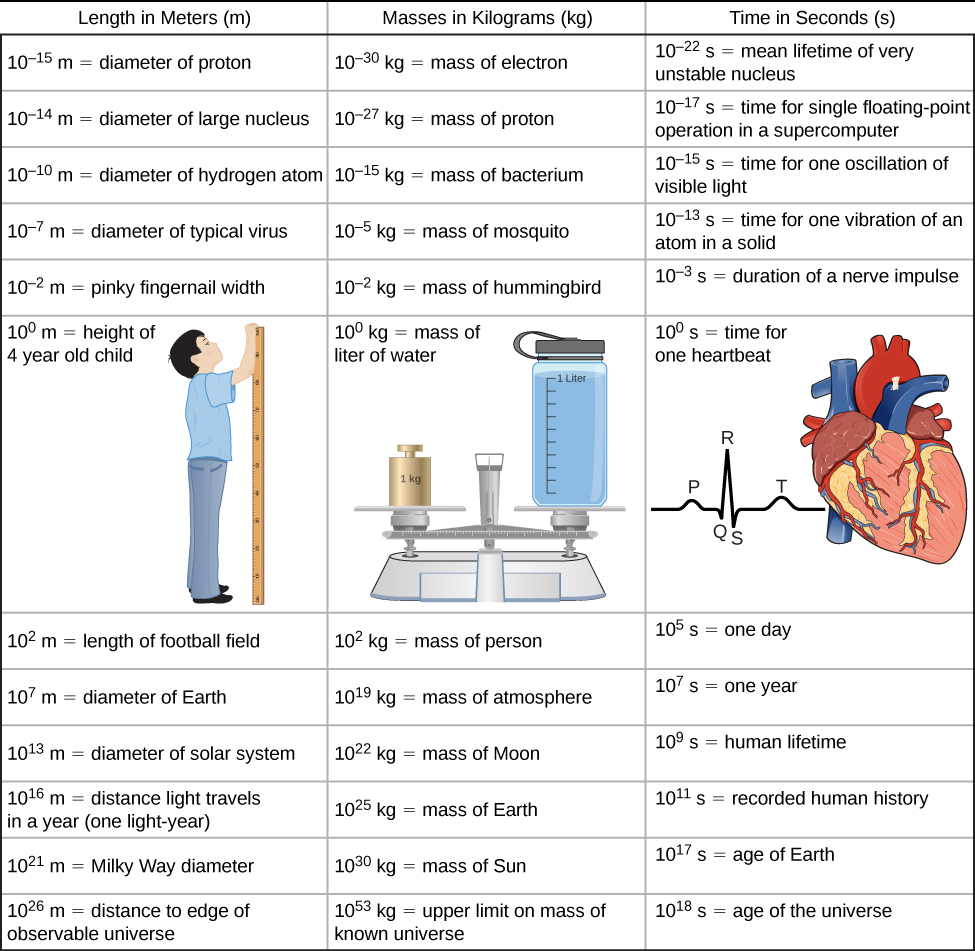
\includegraphics[scale=.7]{./figures/physfig1.jpeg  }
            \end{center}
        \item \textbf{SI Units: Base and Derived Units}
            \bigbreak \noindent 
            \begin{tabularx}{\textwidth}{|X|X|}
                \hline
                ISQ Base Quantity & SI Base Unit \\
                \hline
                Length & meter (m) \\
                Mass & kilogram (kg) \\
                Time & second (s) \\
                Electrical current & ampere (A) \\
                Thermodynamic temperature & kelvin (K) \\
                Amount of substance & mole (mol) \\
                Luminous intensity & candela (cd) \\
                \hline
            \end{tabularx}
            \pagebreak 
        \item \textbf{Metric Prefixes}
            \begin{center}
                \begin{tabularx}{\textwidth}{|X|X|X|X|X|X|}
                    \hline
                    Prefix & Symbol & Meaning & Prefix & Symbol & Meaning \\ 
                    \hline
                    yotta- & Y & $10^{24}$ & yocto- & y & $10^{-24}$ \\
                    zetta- & Z & $10^{21}$ & zepto- & z & $10^{-21}$ \\
                    exa-   & E & $10^{18}$ & atto-  & a & $10^{-18}$ \\
                    peta-  & P & $10^{15}$ & femto- & f & $10^{-15}$ \\
                    tera-  & T & $10^{12}$ & pico-  & p & $10^{-12}$ \\
                    giga-  & G & $10^9$   & nano-  & n & $10^{-9}$  \\
                    mega-  & M & $10^6$   & micro- & $\mu$ & $10^{-6}$ \\
                    kilo-  & k & $10^3$   & milli- & m & $10^{-3}$ \\
                    hecto- & h & $10^2$   & centi- & c & $10^{-2}$ \\
                    deka-  & da & $10^1$  & deci-  & d & $10^{-1}$ \\
                    \hline
                \end{tabularx}
            \end{center}
            \bigbreak \noindent 
        \item \textbf{Base Quantity \& Symbol for Dimension}
            \begin{center}
                \begin{tabularx}{\textwidth}{|X|X|}
                    \hline
                    Base Quantity & Symbol for Dimension \\
                    \hline
                    Length & L \\
                    Mass & M \\
                    Time & T \\
                    Current & I \\
                    Thermodynamic temperature & $\Theta$ \\
                    Amount of substance & N \\
                    Luminous intensity & J \\
                    \hline
                \end{tabularx}
            \end{center}
    \end{itemize}

    \pagebreak 
    \subsubsection{Memorize conversions}
    \begin{itemize}
        \item \textbf{Newton to Pounds}: 
            \begin{align*}
                1N = 0.225lbs
            .\end{align*}
        \item \textbf{Pounds to newtons}
            \begin{align*}
                1lb = 4.448\ N
            .\end{align*}
        \item \textbf{Length/Distance }
            \begin{itemize}
                \item 1 inch (in) = 2.54 centimeters (cm)
                \item 1 centimeter (cm) = 0.393701 inches (in)
                \item 1 foot (ft) = 0.3048 meters (m)
                \item 1 meter (m) = 3.28 feet (ft)
                \item 1 mile (mi) = 1.6 kilometers (km)
                \item 1 kilometer (km) = 0.621371 miles (mi)
            \end{itemize}
    \item \textbf{Weight to mass or mass to weight}
        \begin{itemize}
            \item 1 pound = 0.453592 kilograms.
            \item 1 kilogram = 2.2 pounds.
        \end{itemize}
    \end{itemize}



    \pagebreak 
    \subsubsection{Problems to remember}
    \begin{itemize}
        \item \textbf{Restating mass}: Restate the mass  $1.93 \times 10^{13}$ using a metric prefix such that the resulting numerical value is bigger than one but less than 1000.
            \bigbreak \noindent 
            First, we must restate in terms of grams. Since $1kg = 10^{3}g$, we write
            \begin{align*}
                &1.93 \times 10^{13} \times 10^{3}g \\
                &1.93 \times 10^{16}g
            .\end{align*}
            Since $1Pg = 10^{15}g$, we can write
            \begin{align*}
               1.93 \times 10^{1}Pg 
            .\end{align*}
            Since $16-15 = 1 $
        \item \textbf{Unit conversion}: The distance from the university to home is 10 mi and it usually takes 20 min to drive this distance. Calculate the average speed in meters per second (m/s). (Note: Average speed is distance traveled divided by time of travel.)
        \bigbreak \noindent 
        \textbf{Note:} There are 1609 meters in 1 mile
        \bigbreak \noindent 
        First, we can compute the average speed with the units given $\left(\frac{miles}{minute}\right)$
        \begin{align*}
            \text{Average Speed} = \frac{\text{miles}}{\text{minute}} = \frac{10}{20} = 0.5\ mi/min
        .\end{align*}
        \bigbreak \noindent 
        Now we simply convert to m/s
        \begin{align*}
            &\frac{0.5\ \cancel{mi}}{1\ \cancel{min}} \times \frac{1\ \cancel{min}}{60\ sec} \times \frac{1609\ m}{1\ \cancel{mi}} \\
            &\approx 13 m/s
        .\end{align*}
    \item \textbf{Unit conversion}: The density of iron is  $7.86 g/cm^{3}$ under standard conditions. Convert this to $kg/m^{3}$.
        \begin{align*}
            &\frac{7.86\ g}{1\ cm^{3}} \times \left(\frac{100\ cm}{1\ m}\right)^{3} \times \frac{1\ kg}{1000\ g} \\
            &= \frac{7.86(100^{3})(1\ kg)}{1000(1\ m)} \\
            &=7.86 \cdot 10^{3} kg/m^{3}
        .\end{align*}
    \item \textbf{Proportional}: I found that if I drive my car 110 miles, I use 4 gallons ofgas. If I assume that the relationship between gas guzzled and distance driven is linearly proportional, how many gallons of gas do I use if I drive 275 miles?
        \bigbreak \noindent 
        To answer this lets find the linear equation
        \begin{align*}
            4\ gal = k(100\ mi)
        .\end{align*}
        Where $k$ is some arbitrary factor, Since we know the relationship is proportional, we can write 
        \begin{align*}
            &\frac{X}{4 gal} = \frac{k(275\ mi)}{k(110\ mi)} \\
            &X=10\ gal
        .\end{align*}

    \end{itemize}

    \pagebreak 
    \subsection{Chapter 2: Vectors}

    \smallbreak \noindent
    \subsubsection{Vocabulary}
    \begin{itemize}
        \item Many familiar physical quantities can be specified completely by giving a single number and the appropriate unit. For example, “a class period lasts 50 min” or “the gas tank in my car holds 65 L” or “the distance between two posts is 100 m.” A physical quantity that can be specified completely in this manner is called a \textbf{scalar quantity}. Scalar is a synonym of “number.” Time, mass, distance, length, volume, temperature, and energy are examples of \textbf{scalar quantities}.
        \item possible. Physical quantities specified completely by giving a number of units (magnitude) and a direction are called \textbf{vector quantities}. Examples of vector quantities include displacement, velocity, position, force, and torque.
    \end{itemize}

    \pagebreak 
    \subsubsection{Definitions and theorems (and important things)}
    \begin{itemize}
        \item Vectors (vector quantities) have a \textbf{number of units (magnitude)}, and a \textbf{direction}
        \item \textbf{Algebraic Operations with vectors}
            \begin{itemize}
                \item We can \textbf{add or subtract} two vectors
                \item we can \textbf{multiply} a vector by a scalar or by another vector
                \item We \textbf{cannot} divide by a vector. The operation of division by a vector is not defined.
            \end{itemize}
        \item \textbf{Vector Notation}: We denote a vector with a bold face letter with an arrow above it. For example
            \begin{align*}
                \vec{\textbf{V}}
            .\end{align*}
        \item \textbf{Displacement}: General term used to describe change in position.
        \item \textbf{The magnitude of a vector is the length of the arrow used to represent it}

        \item \textbf{Vector relations}
            \fig{.8}{./figures/vectorimage1.jpeg}

        \item \textbf{Scalars}: When a vector $\vec{A}$ is multiplied by a positive scalar $\alpha$, the result is a new vector $\vec{B}$ that is parallel to $\vec{A}$:
            \begin{align*}
                \vec{\textbf{B}} = \alpha \vec{\textbf{A}}
            .\end{align*}
            The magnitude of this new vector $\vec{\textbf{B}}$ is 
            \begin{align*}
                B = |\alpha|A
            .\end{align*}
            Where $B$ is the magnitude of $\vec{\textbf{B}} $ and $A$ is the magnitude of $\vec{\textbf{A}} $ 
        \item \textbf{Anti parallel vectors (opposing directions)}: Suppose we have two vectors $\vec{\textbf{A}}$ and $\vec{\textbf{B}}$ of equal magnitude. If there are antiparallel, we write
            \begin{align*}
                \vec{\textbf{A}} = -\vec{\textbf{B}} 
            .\end{align*}
        \item The vector sum of two (or more) vectors is called the \textbf{resultant vector} or, for short, the \textbf{resultant}
        \item The vector obtained by adding two vectors is called the \textbf{resultant}
        \item \textbf{Vector Laws }
            \begin{itemize}
                \item \textbf{Communitive law}: $\vec{A} + \vec{B} &= \vec{B} + \vec{A}$
                \item \textbf{Assosiative law}: $(\vec{A} + \vec{B}) + \vec{C} &= \vec{A} + (\vec{B} + \vec{C})$ 
                \item \textbf{Distributive law}: $\alpha_1 \vec{A} + \alpha_2 \vec{A} = (\alpha_1 + \alpha_2)\vec{A}$
            \end{itemize}
        \item \textbf{Vector addition}
            \begin{align*}
               \vec{\textbf{A}} + \vec{\textbf{B}} 
            .\end{align*}
            When two vectors are parallel, we can simply sum their magnitudes. However, if the vectors lie in different directions, the approach for vector addition involves finding their $x$ and $y$ components, summing them and then finding the magnitude. 
        \item \textbf{Vector Subtraction}
            \begin{align*}
                \vec{\textbf{A}} + (-\vec{\textbf{B}})
            .\end{align*}
            \bigbreak \noindent 
            When two vectors are aligned but point in exactly opposite directions, you can subtract their magnitudes (assuming you define one direction as positive and the other as negative) to find the net effect. This is a specific case of adding magnitudes where the direction is implicitly considered through subtraction.
        \item \textbf{Unit Vector notation}:  A unit vector in a normed vector space is a vector of length 1. We declare unit vectors with a hat instead of an arrow, consider the following example
            \begin{align*}
                \hat{\textbf{u}}
            .\end{align*}
            We usually denote the unit vector along the positive x-axis $\hat{i}$, the unit vector along the positive y-axis $\hat{j}$, and the unit vector along the positive z-axis $\hat{k}$
        \item \textbf{Unit vector example}: For example, instead of saying vector $\vec{D}_{AB}$ has a magnitude of $6.0\,\text{km}$ and a direction of northeast, we can introduce a unit vector $\hat{u}$ that points to the northeast and say succinctly that $\vec{D}_{AB} = (6.0\,\text{km})\hat{u}$. Then the southwesterly direction is simply given by the unit vector $-\hat{u}$. In this way, the displacement of $6.0\,\text{km}$ in the southwesterly direction is expressed by the vector
            \begin{align*}
                    \vec{D}_{BA} = (-6.0\,\text{km})\hat{u}.
            .\end{align*}
        \item \textbf{Parallelogram rule for resultant or difference vectors in two dimensions.}:
            \bigbreak \noindent 
            \fig{.8}{./figures/res.jpeg}
            \bigbreak \noindent 
            It follows from the parallelogram rule that neither the magnitude of the resultant vector nor the magnitude of the difference vector can be expressed as a simple sum or difference of magnitudes A and B, because the length of a diagonal cannot be expressed as a simple sum of side lengths.
        \item \textbf{tail-to-head geometric construction}
            \bigbreak \noindent 
            \fig{.8}{./figures/res2.jpeg}
        \item \textbf{Vector $x$ and $y$ components}: The $x$ component can be denoted, $\vec{A_{x}}$ the $y$ component can be denoted $\vec{A_{y}}$. Thus, the vector can be represented as
            \begin{align*}
                &\vec{A} = \vec{A_{x}} + \vec{A_{y}}
            .\end{align*}
        \item \textbf{Unit vectors of the axes}:     It is customary to denote the positive direction on the $x$-axis by the unit vector $\hat{i}$ and the positive direction on the $y$-axis by the unit vector $\hat{j}$. Unit vectors of the axes, $\hat{i}$ and $\hat{j}$, define two orthogonal directions in the plane. The $x$- and $y$- components of a vector can now be written in terms of the unit vectors of the axes:
            \bigbreak \noindent 
               \begin{equation}
                    \begin{cases}
                        \vec{A}_{x} &= A_{x}\hat{i}  \\
                         \vec{A}_{y} &= A_{y}\hat{j}  
                    \end{cases}
                \end{equation}
        \item \textbf{Component form of a vector}:
            \begin{align*}
                \vec{A} = A_{x}\hat{i} + A_{y}\hat{j}
            .\end{align*}
        \item \textbf{Finding components given initial and terminal points}: If we know the coordinates $b(x_b, y_b)$ of the origin point of a vector (where $b$ stands for "beginning") and the coordinates $e(x_e, y_e)$ of the end point of a vector (where $e$ stands for "end"), we can obtain the scalar components of a vector simply by subtracting the origin point coordinates from the end point coordinates:
            \begin{align*}
                A_x &= x_e - x_b  \\
                A_y &= y_e - y_b
            .\end{align*}
        \item \textbf{Magnitude $A$ of a vector with components $A_{x}$ and $A_{y}$}
            \begin{align*}
               &A^{2}  = A_{x}^{2} + A_{y}^{2} \\
               &A = \sqrt{A_{x}^{2} + A_{y}^{2}}
            .\end{align*}
            This equation works even if the scalar components of a vector are negative.
        \item \textbf{Finding theta for a vector (used for direction angles)}
            \begin{align*}
                \tan{\theta } = \frac{A_{y}}{A_{x}}
            .\end{align*}
        \item \textbf{Direction angles for vectors in the first}:
        \item \textbf{Direction angles for vectors in the second quadrant}:
            \begin{align*}
                \theta_{A} = \theta 
            .\end{align*}
        \item \textbf{Direction angles for vectors in the second quadrant}:
            \begin{align*}
                \theta_{A} = 180 - \theta 
            .\end{align*}
        \item \textbf{Direction angles for vectors in the second quadrant}:
            \begin{align*}
                \theta_{A} = 180 + \theta 
            .\end{align*}
        \item \textbf{Direction angles for vectors in the fourth quadrant}:
            \begin{align*}
                \theta_{A} = 360 - \theta 
            .\end{align*}
        \item \textbf{Finding $A_{x}$ and $A_{y}$  when the magnitude and direction angle are known}
        \begin{equation}
            \begin{cases}
                &A_{x} = A\cos{\theta_{A}} \\
                &A_{y} = A\sin{\theta_{A}} \\
            \end{cases}
        \end{equation}
        \item \textbf{Polar form}
            \begin{align*}
                &x = r\cos{\varphi} \\
                &y = r\sin{\varphi}
            .\end{align*}
        \item \textbf{Three dimensional plane}
            \bigbreak \noindent 
            \fig{.8}{./figures/zaxis.jpeg}
        \item \textbf{$z$ component of a vector}:
            \begin{align*}
                \vec{A}_{z} = A_{z}\hat{k} 
            .\end{align*}
            Where $A_{z}$ is given by 
            \begin{align*}
                z_{e} - z_{b}
            .\end{align*}
        \item \textbf{Vector in three dimensions}: A vector in three-dimensional space is the vector sum of its three vector component. 
            \begin{align*}
                \vec{A} = A_x \hat{i} + A_y \hat{j} + A_z \hat{k}.
            .\end{align*}
        \item \textbf{Magnitude of a vector in three dimensions}
            \begin{align*}
                A = \sqrt{A_x^2 + A_y^2 + A_z^2}.
            .\end{align*}
        \item \textbf{Null vector}: Denoted by 
            \begin{align*}
                \vec{0}
            .\end{align*}
            Has all components 0. Thus, 
            \begin{align*}
                \vec{0} = 0\hat{i} + 0\hat{j} + 0\hat{k}
            .\end{align*}
            Thus, it has no direction and no length
        \item Two vectors $\vec{A}$ and $\vec{B}$ are \textbf{equal vectors} if and only if their difference is the null vector:
        Hence, we can write $\vec{A} = \vec{B}$ if and only if the corresponding components of vectors $\vec{A}$ and $\vec{B}$ are equal:
        \[
        \vec{A} = \vec{B} \Leftrightarrow
        \left\{
            \begin{array}{l}
                A_x = B_x \\
                A_y = B_y \\
                A_z = B_z
            \end{array}
        \right.
        \]
    \item \textbf{Components of a resultant vector}:
        \begin{equation}
            \begin{cases}
                R_{x} = A_{x}  + B_{x} \\
                R_{y} = A_{y}  + B_{y} \\
                R_{z} = A_{z}  + B_{z} 
            \end{cases}
        \end{equation}

    \item \textbf{components of a resultant of many vectors}: if we are to sum up $N$ vectors $\vec{F}_1, \vec{F}_2, \vec{F}_3, \ldots, \vec{F}_N$, where each vector is $\vec{F}_k = F_{kx}\hat{i} + F_{ky}\hat{j} + F_{kz}\hat{k}$, the resultant vector $\vec{F}_R$ is
           \begin{equation}
                \begin{cases}
                    F_{R_{x}} = \summation{N}{k=1}\ F_{kx}\ = F_{1x} + F_{2x} + F_{3x} + ... + F_{Nx} \\
                    F_{R_{y}} = \summation{N}{k=1}\ F_{ky}\ = F_{1y} + F_{2y} + F_{3y} + ... + F_{Ny} \\
                    F_{R_{z}} = \summation{N}{k=1}\ F_{kz}\ = F_{1z} + F_{2z} + F_{3z} + ... + F_{Nz} \\
                \end{cases}
            \end{equation}
        With the component form 
        \begin{align*}
            \vec{F_{R}} = F_{R_{x}}\hat{i} + F_{R_{y}}\hat{j} + F_{R_{z}}\hat{k}
        .\end{align*}
    \item \textbf{Finding unit vector (Direction) of some vector}: Suppose we have some vector $\vec{V}$. Then 
        \begin{align*}
            \hat{V} = \frac{\vec{V}}{V}
        .\end{align*}
    \item \textbf{Dot product}
        \begin{align*}
            \vec{A} \cdot \vec{B} = AB\cos{\varphi} 
        .\end{align*}
        Where $\varphi$ is the angle between the vectors
    \item \textbf{Dot product of two parallel vectors}
        \begin{align*}
            \vec{A} \cdot \vec{B} = AB\cos{0^{\circ}} = AB
        .\end{align*}
    \item \textbf{Dot product of two anti-parallel vectors}
        \begin{align*}
            \vec{A} \cdot \vec{B} = AB\cos{180^{\circ}} = -AB
        .\end{align*}
    \item \textbf{Dot product of two orthogonal vectors}
        \begin{align*}
            \vec{A} \cdot \vec{B} = AB\cos{90^{\circ}} =  0
        .\end{align*}
    \item \textbf{Dot product of a vector with itself}
        \begin{align*}
            \vec{A} \cdot \vec{A} = AA\cos{0} = A^{2}
        .\end{align*}
    \item \textbf{Dot products of unit vectors}: Scalar products of the unit vector of an axis with other unit vectors of axes always vanish (equals 0) because these unit vectors are orthogonal:
    \item \textbf{Dot product of the same unit vector}: The dot product of the same unit vector is 1
        \begin{align*}
            \hat{i} \cdot \hat{i} = i^{2} = 1
        .\end{align*}
    \item \textbf{Using dot product to find scalar x-component}
        \begin{align*}
            \vec{A} \cdot \hat{i} = \norm{\vec{A}} \norm{\hat{i}}\cos{\theta_{A}} = A\cos{\theta_{A}}= A_{x}
        .\end{align*}
    \item \textbf{Using dot product to find scalar y-component}
        \begin{align*}
            \vec{A} \cdot \hat{j} = \norm{\vec{A}} \norm{\hat{j}}\cos{(90^{\circ} -\theta_{A})}= A\sin{\theta_{A}} = A_{y}
        .\end{align*}
    \item \textbf{Trig complementary angles}: For a right angle triangle, the sine of the complemenary angle is the cosine of the angle. And vice versa
        \begin{align*}
            &\sin{90-\theta} = \cos{\theta} \\
            &\cos{90-\theta} = \sin{\theta}
        .\end{align*}
    \item \textbf{Dot product second method of computation}
        \begin{align*}
            \vec{A} \cdot \vec{B} = A_{x}B_{x} + A_{y}B_{y} + A_{z}B_{z}
        .\end{align*}
    \item \textbf{Equation for $\cos{(\varphi)}$}
        \begin{align*}
            \cos{(\varphi)} = \frac{\vec{A} \cdot \vec{B}}{AB}
        .\end{align*}
    \item The \textbf{Si unit for work} is the joule (J), where 
        \begin{align*}
            1\ \text{J} = 1\ \text{N} \cdot \text{m} 
        .\end{align*}
    \item \textbf{The Work of a Force}: When force $\vec{F}$ pulls on an object and when it causes its displacement $\vec{D}$, we say the force performs work. The amount of work the force does is the scalar product $\vec{F} \cdot \vec{D}$.
    \item \textbf{Cross Product (Vector Product)}: 
        The vector product of two vectors $\vec{A}$ and $\vec{B}$ is denoted by $\vec{A} \times \vec{B}$ and is often referred to as a cross product. The vector product is a vector that has its direction perpendicular to both vectors $\vec{A}$ and $\vec{B}$. In other words, vector $\vec{A} \times \vec{B}$ is perpendicular to the plane that contains vectors $\vec{A}$ and $\vec{B}$. The magnitude of the vector product is defined as
        \begin{equation}
            \lVert \vec{A} \times \vec{B} \rVert = AB \sin \varphi,
        \end{equation}
        where angle $\varphi$, between the two vectors, is measured from vector $\vec{A}$ (first vector in the product) to vector $\vec{B}$ (second vector in the product), as indicated in Figure 2.29, and is between $0^\circ$ and $180^\circ$.
    \item     The \textbf{vector product vanishes} for pairs of vectors that are either \textbf{parallel} ($\varphi=0^\circ$) or \textbf{antiparallel} ($\varphi=180^\circ$) because $\sin 0^\circ = \sin 180^\circ = 0$.
    \item The cross product is \textbf{anti-communitive}
        \begin{align*}
            \vec{A} \times \vec{B} = -\vec{B} \times \vec{A}.
        .\end{align*}
    \item \textbf{Torque}: Denoted with the greek letter "tau" is the vector product of the distance between the pivot to force with the force:
        \begin{align*}
            \vec{\tau} = \vec{R} \times \vec{F}
        .\end{align*}
    \item \textbf{the cross product has the following distributive property:}
        \begin{align*}
            \vec{A} \times (\vec{B} + \vec{C}) = \vec{A} \times \vec{B} + \vec{A} \times \vec{C}
        .\end{align*}
    \item \textbf{Cross product of the same unit vectors}: The cross product of the same unit vectors is 0
    \item \textbf{Cross product between unit vectors}
        \begin{equation}
            \begin{cases}
                \hat{i} \times \hat{j} = +\hat{k} \\
                \hat{j} \times \hat{i} = -\hat{k} \\
                \hat{j} \times \hat{k} = +\hat{i} \\
                \hat{k} \times \hat{j} = -\hat{i} \\
                \hat{k} \times \hat{i} = +\hat{j} \\
                \hat{i} \times \hat{k} = -\hat{j}
            \end{cases}
        \end{equation}
        \bigbreak \noindent 
        \textbf{Notice:} The cross product of two different unit vectors is always a third unit vector.
    \item \textbf{Computation of the cross product}:
        \begin{align*}
            \vec{C} = \vec{A} \times \vec{B} = (A_yB_z - A_zB_y)\hat{i} + (A_zB_x - A_xB_z)\hat{j} + (A_xB_y - A_yB_x)\hat{k}
        .\end{align*}
        \pagebreak 
    \item \textbf{Average Velocity}: Velocity is the \textbf{vector quantity} of speed plus the direction. Velocity is 
        \begin{align*}
            \vec{v} &=\frac{\text{Displacement}}{Time} = \frac{\norm{\vec{d}}}{t}
        .\end{align*}
        Where $\norm{\vec{d}}$ is the magnitude of the displacement vector, and $t$ is the total elapsed time.
    \item To describe the position (location) of something, we give its distance from the orgin and its direction. This vector quantity is called the \textbf{position vector}, Denoted
        \begin{align*}
            \vec{r}
        .\end{align*}
        \bigbreak \noindent 
    \begin{figure}[ht]
        \centering
        \incfig{try2}
        \label{fig:try2}
    \end{figure}
    \item \textbf{Displacement} is defined as the change in the position vector. The final position vector minus the initial position vector
        \begin{align*}
            \Delta \vec{r} = \vec{r}_{f} - \vec{r}_{i}
        .\end{align*}
    \begin{figure}[ht]
        \centering
        \incfig{hellowrold}
        \label{fig:hellowrold}
    \end{figure}






    \end{itemize}

    \pagebreak 
    \subsubsection{Problems to remember}
    \begin{itemize}
        \textbf{Unit vectors}: A long measuring stick rests against a wall in a physics laboratory with its 200-cm end at the floor. A ladybug lands on the 100-cm mark and crawls randomly along the stick. It first walks 15 cm toward the floor, then it walks 56 cm toward the wall, then it walks 3 cm toward the floor again. Then, after a brief stop, it continues for 25 cm toward the floor and then, again, it crawls up 19 cm toward the wall before coming to a complete rest (Figure 2.8). Find the vector of its total displacement and its final resting position on the stick.
        \bigbreak \noindent 
        If we choose the direction along the stick toward the floor as the direction of unit vector $\hat{u}$, then the direction toward the floor is $+\hat{u}$ and the direction toward the wall is $-\hat{u}$. The ladybug makes a total of five displacements:
        \begin{align*}
        &\vec{D}_1 = (15\,\text{cm})(+\hat{u}), \quad \vec{D}_2  \\
        &= (56\,\text{cm})(-\hat{u}), \quad \vec{D}_3  \\
        &= (3\,\text{cm})(+\hat{u}), \quad \vec{D}_4  \\
        &= (25\,\text{cm})(+\hat{u}), \quad \text{and} \quad \vec{D}_5  \\
        &= (19\,\text{cm})(-\hat{u}).
    .\end{align*}
    The total displacement $\vec{D}$ is the resultant of all its displacement vectors.
    \bigbreak \noindent 
    The resultant of all the displacement vectors is
    \begin{align*}
        &\vec{D} = \vec{D}_1 + \vec{D}_2 + \vec{D}_3 + \vec{D}_4 + \vec{D}_5  \\
        &= (15\,\text{cm})(+\hat{u}) + (56\,\text{cm})(-\hat{u}) + (3\,\text{cm})(+\hat{u}) + (25\,\text{cm})(+\hat{u}) + (19\,\text{cm})(-\hat{u})  \\
        &= (15 - 56 + 3 + 25 - 19)\,\text{cm}\,\hat{u} = -32\,\text{cm}\,\hat{u}
    .\end{align*}
    In this calculation, we use the distributive law. The result reads that the total displacement vector points away from the 100-cm mark (initial landing site) toward the end of the meter stick that touches the wall. The end that touches the wall is marked 0 cm, so the final position of the ladybug is at the $(100 - 32)\,\text{cm} = 68\,\text{cm}$ mark.
    \end{itemize}

    \pagebreak 
    \subsection{Chapter 3: Motion along a straight line}
    \bigbreak \noindent 
    \subsubsection{Definitions and theorems}
    \begin{itemize}
        \item \textbf{Kinematics} is a subfield of physics, developed in classical mechanics, that describes the motion of points, bodies, and systems of bodies without considering the forces that cause them to move
        \item \textbf{Displacement}: Displacement $\Delta x$ is the change in position of an object:
            \begin{align*}
                \Delta x = x_f - x_0,
            .\end{align*}
            where $\Delta x$ is displacement, $x_f$ is the final position, and $x_0$ is the initial position.
        \item We define total displacement $\Delta x_{\text{Total}}$, as the sum of the individual displacements, and express this mathematically with the equation
            \begin{align*}
                \Delta x_{\text{Total}} = \sum \Delta x_i
            .\end{align*}
        \item \textbf{the distance traveled} is the sum of the magnitudes of the individual displacements:
            \begin{align*}
                x_{\text{total}} = \summation{n}{i=1}\ \Delta x_{i}
            .\end{align*}
        \item If the details of the motion at each instant are not important, the rate is usually expressed as the \textbf{average velocity}. If  $x_{1}$ and  $x_{2} $ are the positions of an object at times  $t_{1} $ and  $t_{2}$ , respectively, then 
            \begin{align*}
                \text{Average Velocity } =\ &\bar{v} =  \frac{\text{Displacement between two points}}{\text{Time needed to make the displacement}} \\
                &\bar{v} = \frac{\Delta x}{\Delta t} = \frac{x_{2} - x_{1}}{t_{2} - t_{1}}
            .\end{align*}
        
            This vector quantity is simply the total displacement between two points divided by the time taken to travel between them. The time taken to travel between two points is called the \textbf{elapsed time} $\Delta t$
        \item The \textbf{instantaneous velocity} of an object is the limit of the average velocity as the elapsed time approaches zero, or the derivative of $x$ with respect to $t$:
            \begin{align*}
                v(t) &= \lim\limits_{\Delta t \to 0}{\frac{f(t + \Delta t) - f(t)}{\Delta t}} \\
                 &= \frac{d}{dt}x(t).
            .\end{align*}
        \item We can calculate the \textbf{average speed} by finding the total distance traveled divided by the elapsed time:
            \begin{align*}
                \text{Average speed } = \bar{s} = \frac{\text{Total distance}}{\text{Elapsed time}}.
            .\end{align*}
        \item we can calculate the \textbf{instantaneous speed} from the magnitude of the instantaneous velocity:
            \begin{align*}
                \text{instantaneous speed } = \bigg\lvert v(t) \bigg\rvert
            .\end{align*}
        \item \textbf{Calculating Instantaneous Velocity}
            When calculating instantaneous velocity, we need to specify the explicit form of the position function $x(t)$. If each term in the $x(t)$ equation has the form of $A t^n$ where $A$ is a constant and $n$ is an integer, this can be differentiated using the power rule to be:
            \begin{align*}
                \frac{d(At^{n})}{dt}= Ant^{n-1}
            .\end{align*}
        \item \textbf{Average acceleration} is the rate at which velocity changes:
            \begin{align*}
                \bar{a} = \frac{\Delta v}{\Delta t} = \frac{v_f - v_0}{t_f - t_0},
            .\end{align*}
            where $\bar{a}$ is average acceleration, $v$ is velocity, and $t$ is time. (The bar over the $a$ means average acceleration.)
            \bigbreak \noindent 
            \textbf{Note:} acceleration occurs when velocity changes in magnitude (an increase or decrease in speed) or in direction, or both.
               \item \textbf{Acceleration as a vector:} Acceleration is a vector in the same direction as the change in velocity,  $\Delta v$ . Since velocity is a vector, it can change in magnitude or in direction, or both. Acceleration is, therefore, a change in speed or direction, or both.
         \bigbreak \noindent 
         Keep in mind that although acceleration is in the direction of the change in velocity, it is not always in the direction of motion. When an object slows down, its acceleration is opposite to the direction of its motion. Although this is commonly referred to as deceleration
        \item \textbf{Distance over constant acceleration}
            \begin{align*}
                d = \frac{1}{2}at^{2} 
            .\end{align*}
            Where $a$ is the acceleration, and $t$ is the time
        \item \textbf{instantaneous acceleration}
            \begin{align*}
            a(t) = \frac{d}{dt}v(t)
            .\end{align*}
        \item \textbf{Derivative of velocity function}: Suppose we have some function 
            \begin{align*}
                v(t) = (20 m/s) t - (10 m/s^{2})t^{2}
            .\end{align*}
            When we find the acceleration function, we are taking the derivative of the velocity function. Thus, we are finding the change in velocity with respect to time. Consequently, our terms become
            \begin{align*}
                a(t) = 20 m/s^{2} - (10m/s^{3})t
            .\end{align*}
            \textbf{Notice:} How we are dividing by an additional unit of time, thus the exponents for our seconds increases by one.
        \item \textbf{Simplified notation}: If we take initial time to be zero, and final quantitys without subscript, then we have 
            \begin{align*}
               &\Delta t = t\\
                &\Delta x = x - x_{0}\\
                &\Delta v = v- v_{0}\\
            .\end{align*}
        \item \textbf{Assumption of constant acceleration}: This assumption allows us to avoid using calculus to find instantaneous acceleration. Since acceleration is constant, the average and instantaneous accelerations are equal—that is,
            \begin{align*}
                \bar{a} = a = \text{constant}
            .\end{align*}
            Thus, we can use the symbol $a$ for acceleration at all times.
        \item \textbf{Final Position function} 
            \begin{align*}
                x = x_{0}  + \bar{v}t
            .\end{align*}
        \item \textbf{Average velocity under constant acceleration}
            \begin{align*}
                \bar{v} = \frac{v_{0} + v}{2} \quad \text{(Constant $a$)}
            .\end{align*}
            This reflects the fact that when acceleration is constant, $\bar{v}$ is just the simple average of the initial and final velocities.
        \item \textbf{Final Velocity function under constant acceleration}
            \begin{align*}
                v = v_{0} + at \quad \text{(Constant $a$)}
            .\end{align*}
        \item \textbf{Equation for final position under constant acceleration}
            \begin{align*}
                x = x_{0} +v_{0}t + \frac{1}{2}at^{2} \quad \text{(Constant $a$)}
            .\end{align*}
            When initial position and velocity are both zero, we have
            \begin{align*}
                x =  \frac{1}{2}at^{2} \quad \text{(Constant $a$)}
            .\end{align*}
        \item \textbf{relationships seen in final position under constant acceleration equation}
            \begin{itemize}
                \item Displacement depends on the square of the elapsed time when acceleration is not zero.
                \item If acceleration is zero, then initial velocity equals average velocity \(v_0 = \bar{v}\), and \(x = x_0 + v_0t + \frac{1}{2}at^2\) becomes \(x = x_0 + v_0t\).
            \end{itemize}
        \item \textbf{Final velocity equation (no time required)}
            \begin{align*}
                v^{2} = v_{0}^{2} + 2a(x-x_{0}) \quad \text{(Constant $a$)}
            .\end{align*}
        \item \textbf{additional insights into the general relationships among physical quantities:}
            \begin{itemize}
                \item The final velocity depends on how large the acceleration is and the distance over which it acts.
                \item For a fixed acceleration, a car that is going twice as fast doesn’t simply stop in twice the distance. It takes much farther to stop. (This is why we have reduced speed zones near schools.)
            \end{itemize}
        \item \textbf{acceleration in terms of velocities and displacement}
            \begin{align*}
                a  = \frac{v^{2} - v_{0}^{2}}{2(x-x_{0})}
            .\end{align*}
        \item \textbf{two-body pursuit problems}
            \begin{itemize}
                \item Find equations of motion for both bodies (with the same parameter)
                \item eliminate the parameter
                \item plug in knowns to solve for the unknown
            \end{itemize}



    \end{itemize}

    \pagebreak 
    \subsubsection{Problems to remember}

    \pagebreak 
    \unsect{Calculus III}

    \bigbreak \noindent 
    \subsection{Chapter 1: Parametric equations and polar coordinates}
    \subsubsection{Definitions and Theorems} 
    \begin{itemize}
        \item \textbf{Parametric equations, parameter}: 
            If \( x \) and \( y \) are continuous functions of \( t \) on an interval \( I \), then the equations
            \[ x = x(t) \quad \text{and} \quad y = y(t) \]
            are called \textbf{parametric equations} and \( t \) is called the \textbf{parameter}. 
        \item \textbf{Parametric Curve}: The set of points \( (x, y) \) obtained as \( t \) varies over the interval \( I \) is called the graph of the parametric equations. The graph of parametric equations is called a \textbf{parametric curve} or plane curve, and is denoted by \( C \).
        \item \textbf{Eliminating the parameter:} This allows us to rewrite the two equations as a single equation relating the variables x and y. Then we can apply any previous knowledge of equations of curves in the plane to identify the curve. 
            \begin{itemize}
                \item Solve one of the equations for $t$
                \item Plug the equation for $t$ into the equation still in terms of $t$
                \item Sketch the curve on the interval $I$
            \end{itemize}
        \item \textbf{Domain consideration when graphing by eliminating the parameter}: Suppose we have the equations 
            \begin{align*}
                &x = 2t^{2} \\
                &y = t^{4} + 1
            .\end{align*}
            If we solve $x$ for $t$, we get 
            \begin{align*}
                 t = \pm \sqrt{\frac{1}{2}x}
            .\end{align*}
            We see that the domain of $t$ is restricted to  $t \geq 0$, thus, the graph of this equation will only have the positive side.
        \item \textbf{Parameterizing a curve} is when we start with the equation of a curve and determine a pair of parametric equations for that curve.
            \begin{itemize}
                \item To find the first Parameterization, Define $x(t) = t $ and $y(t)$ as the function given, with $t$ instead of x 
                \item Verify there is no restriction on the domain of the original graph. Thus there is no restriction on the values of $t $
            \end{itemize}
            \begin{itemize}
                \item To find the second parameterization, choose some function for $x(t)$. Ensure that the domain is the set of all real numbers
                \item Plug $x(t)$ into the original function and solve to get $y(t)$
            \end{itemize}
        \item \textbf{Parametric equations for a cylcloid}
            \begin{align*}
                x(t) = a(t-\sin{t}), \quad y(t) = a(1-\cos{t})
            .\end{align*}
        \item \textbf{The general parametric equations for a hypocycloid are:}
            \begin{align*}
                &x(t) = (a-b)\ \cos{t} + b \cos{\left(\frac{a-b}{b}\right)}t \\
                &y(t) = (a-b)\ \sin{t} + b \sin{\left(\frac{a-b}{b}\right)}t \\
            .\end{align*}
        \item \textbf{Derivatives of Parametric Equations}:
            Consider the plane curve defined by the parametric equations \( x = x(t) \) and \( y = y(t) \). Suppose that \( x'(t) \) and \( y'(t) \) exist, and assume that \( x'(t) \neq 0 \). Then the derivative \( \frac{dy}{dx} \) is given by
            \[
                \frac{dy}{dx} = \frac{\frac{dy}{dt}}{\frac{dx}{dt}} = \frac{y'(t)}{x'(t)}.
            \]
        \item \textbf{Second order derivatives of parametric functions}
            \begin{align*}
                \frac{d^{2}y}{dx^{2}} = \frac{d}{dx}\left(\frac{dy}{dx}\right) = \frac{\left(\frac{d}{dt}\right)\left(\frac{dy}{dx}\right)}{\frac{dx}{dt}}
            .\end{align*}
        \item \textbf{Integral involving parametric equations}
            Consider the non-self-intersecting plane curve defined by the parametric equations
            \[
                x = x(t), \quad y = y(t), \quad a \leq t \leq b
            \]
            and assume that \( x(t) \) is differentiable. The area under this curve is given by
            \[
                A = \int_{a}^{b} y(t) x'(t) \, dt.
            \]
        \item \textbf{Arc Length of a Parametric Curve}:
            Consider the plane curve defined by the parametric equations
            \[
                x = x(t), \quad y = y(t), \quad t_1 \leq t \leq t_2
            \]
            and assume that \( x(t) \) and \( y(t) \) are differentiable functions of \( t \). Then the arc length of this curve is given by
            \[
                s = \int_{t_1}^{t_2} \sqrt{\left(\frac{dx}{dt}\right)^2 + \left(\frac{dy}{dt}\right)^2} \, dt.
            \]
            Or simply
            \begin{align*}
                s = \int_{a}^{b}\ \sqrt{1 + \left(\frac{dy}{dx}\right)^{2}}\ dx
            .\end{align*}
        \item \textbf{Surface area for a parametric curve}:
            The analogous formula for a parametrically defined curve is
            \[
                S = 2\pi \int_{a}^{b} y(t) \sqrt{(x'(t))^2 + (y'(t))^2} \, dt
            \]
            provided that \( y(t) \) is not negative on \([a, b]\).
        \item \textbf{Parametric equations for a circle (with $(h,k) = (0,0)$)}
            \begin{align*}
                &x(t) = r\cos{(t)} \\
                &y(t) = r\sin{(t)}
            .\end{align*}
            For $0 \leq t \leq 2\pi $
        \item \textbf{Parametric equations for the upper half of a semi-circle (with $(h,k) = (0,0)$)}
            \begin{align*}
                &x(t) = r\cos{(t)} \\
                &y(t) = r\sin{(t)}
            .\end{align*}
            For $0 \leq t \leq \pi $
        \item \textbf{Parametric equations for the lower half of a semi-circle (with $(h,k) = (0,0)$)}
            \begin{align*}
                &x(t) = r\cos{(t)} \\
                &y(t) = r\sin{(t)}
            .\end{align*}
            For $\pi \leq t \leq 2\pi $
        \item \textbf{Note: A graph has a horizontal tangent line when the derivative equals zero.}
        \item \textbf{Note: A graph has a vertical tangent line when the derivative does not exist}
        \item \textbf{Converting Points between Coordinate Systems}: 
            Given a point \( P \) in the plane with Cartesian coordinates \((x, y)\) and polar coordinates \((r, \theta)\), the following conversion formulas hold true:
            \begin{align*}
                x = r \cos \theta \quad \text{and} \quad y = r \sin \theta,
            .\end{align*}
            \begin{align*}
                r^2 = x^2 + y^2 \quad \text{and} \quad \tan \theta = \frac{y}{x}.
            .\end{align*}
            These formulas can be used to convert from rectangular to polar or from polar to rectangular coordinates.
        \item \textbf{Sometimes finding $\theta$ with the formula is not possible.} Consider the point $P(0,3)$, using the formula $\tan{\theta } = \frac{3}{0}$ is undefined. Instead, we graph the point $(0,3)$ and observe the angle between the $x$ and $y$ axis is $\frac{\pi}{2}$ 
        \item \textbf{The polar representation of a point is not unique.} Every point in the plane has an infinite number of representations in polar coordinates. However, each point in the plane has only one representation in the rectangular coordinate system.
        \item The line segment starting from the center of the graph going to the right (called the positive x-axis in the Cartesian system) is the \textbf{polar axis}. 
        \item The center point is the \textbf{pole}, or origin, of the coordinate system, and corresponds to  $r=0$.
        \item \textbf{If the value of  $r$ is positive}, move that distance along the terminal ray of the angle. \textbf{If it is negative}, move along the ray that is opposite the terminal ray of the given angle.
        \item A \textbf{Polar equation} has the form
            \begin{align*}
                r = f(\theta )
            .\end{align*}
        \item \textbf{Plotting a Curve in Polar Coordinates}
            \begin{enumerate}
                \item Create a table with two columns. The first column is for \( \theta \), and the second column is for \( r \).
                \item Create a list of values for \( \theta \).
                \item Calculate the corresponding \( r \) values for each \( \theta \).
                \item Plot each ordered pair \( (r, \theta) \) on the coordinate axes.
                \item Connect the points and look for a pattern.
            \end{enumerate}
            \pagebreak 
        \item \textbf{Types of polar curves}
     \bigbreak \noindent 
     \begin{tabularx}{\textwidth}{|X|X|X|}
        \hline
        Name & Equation & Example \\
        \hline
        Line passing through the pole with slope $\tan{K}$ & $\theta =K$ & \fig{.5}{./figures/14.png}\\
        \hline
        Circle & $r=a\cos{\theta} + b\sin{\theta} $ & \fig{.5}{./figures/16.png}\\
        \hline
        Spiral& $r=a+b\theta  $&\fig{.5}{./figures/15.png} \\
        \hline
     \end{tabularx}

     \pagebreak \bigbreak \noindent 
      \begin{tabularx}{\textwidth}{|X|X|X|}
        \hline
        Name & Equation & Example \\
        \hline
        Cardioid & \fig{.5}{./figures/20.png} & \fig{.5}{./figures/17.png}\\
        \hline
        Limacon & \fig{.5}{./figures/21.png} & \fig{.5}{./figures/18.png}\\
        \hline
        Rose & \fig{.5}{./figures/23.png}&\fig{.5}{./figures/19.png} \\
        \hline
     \end{tabularx}
     \bigbreak \noindent 
 \item      For the rose, \textbf{If the coefficient of $\theta$ is even}, the graph has twice as many petals as the coefficient. \textbf{If the coefficient of $\theta$ is odd, then the number of petals equals the coefficient.}

     \pagebreak 
    \item \textbf{Graphing a polar curve.}
        \begin{itemize}
            \item Make graph in rectangular system (use $\theta$ as horizontal axis and $r$ as vertical)
            \item Translate over to polar
            \item The circles represent values of $r$
        \end{itemize}
        \item \textbf{Area of a Region Bounded by a Polar Curve}:
             Suppose \( f \) is continuous and nonnegative on the interval \( \alpha \leq \theta \leq \beta \) with \( 0 < \beta - \alpha \leq 2\pi \). The area of the region bounded by the graph of \( r = f(\theta) \) between the radial lines \( \theta = \alpha \) and \( \theta = \beta \) is
                \[ A = \frac{1}{2} \int_{\alpha}^{\beta} [f(\theta)]^2 \, d\theta = \frac{1}{2} \int_{\alpha}^{\beta} r^2 \, d\theta. \]
        \item \textbf{Area between two polar curves}:
            \begin{align*}
                A = \frac{1}{2}\int_{\alpha}^{\beta}\ f(\theta)^{2} -g(\theta )^{2}\ d\theta 
            .\end{align*}
            Where $f(\theta ) \geq g(\theta ) \forall\ \alpha \leq \theta \leq \beta $

        \item \textbf{Bounds of integration for area outside some curve and inside some curve}: We find the bounds of integration the same way we found them for regularo functions, we find the points of intersection by setting the two functions equal to each other
        \item \textbf{Arc Length of a Curve Defined by a Polar Function}:
            Let \( f \) be a function whose derivative is continuous on an interval \( \alpha \leq \theta \leq \beta \). The length of the graph of \( r = f(\theta) \) from \( \theta = \alpha \) to \( \theta = \beta \) is
            \begin{align*}
              &L = \int_{\alpha}^{\beta} \sqrt{[f(\theta)]^2 + [f'(\theta)]^2} \, d\theta \\
              &= \int_{\alpha}^{\beta} \sqrt{r^2 + \left(\frac{dr}{d\theta}\right)^2} \, d\theta. 
          .\end{align*}
        \item \textbf{Absolute value bars}: Consider the integral
            \begin{align*}
                20 \int_{0}^{2\pi}\ \sqrt{\cos^{2}{\left(\frac{\theta }{2}\right)}}\ d\theta 
            .\end{align*}
            If we cancel out the sqrt and square, we must include absulute value bars. This is because $\cos{\left(\frac{\theta }{2}\right)}$ can be negative on the interval $[0,2\pi]$. The integral becomes
            \begin{align*}
                20 \int_{0}^{2\pi}\ \bigg\lvert \cos{\left(\frac{\theta}{2}\right)} \bigg\rvert\ d\theta 
            .\end{align*}
            To solve this, we use symmetry to change the bounds. Because the graph of the polar curve ($10+10\cos{\theta}$) is symmetric, we can integrate instead over the range $0,\pi$, and multiply the result by 2.
        \item \textbf{Derivative of polar equaotion}: Given some function $r=f(\theta )$. We can find the derivative with
            \begin{align*}
                \frac{dy}{dx} = \frac{\frac{dy}{d\theta}}{\frac{dx}{d\theta}} = \frac{\frac{dr}{d\theta }\sin{\theta } + r\cos{\theta }}{\frac{dr}{d\theta }\cos{\theta } - r\sin{\theta}}
            .\end{align*}
        \item \textbf{Find equation of tangent line given $r = f(\theta )$ and point $\theta$}. 
            \begin{itemize}
                \item Find $r$ with given $\theta$.
                \item Plug $r$ into $x=r\cos{\theta }$, $y=r\sin{\theta }$ to get point $P(x,y)$
                \item Find $\frac{dy}{dx}$ of $r=f(\theta)$
                \item Plug in $\theta$ to get slope $m$
                \item Use point slope form to find equation
            \end{itemize}






    \end{itemize}

    \pagebreak 
    \subsubsection{Problems to remember}
    \begin{itemize}
        \item \textbf{Eliminating the parameter:}
            Sometimes it is necessary to be a bit creative in eliminating the parameter. The parametric equations for this example are
            \begin{align*}
                x(t) = 4\cos{t}, \quad y(t) = 3\sin{t}
            .\end{align*}
            \bigbreak \noindent 
            Solving either equation for $t$ directly is not advisable because sine and cosine are not one-to-one functions. However, dividing the first equation by 4 and the second equation by 3 (and suppressing the $t$) gives us
            \begin{align*}
                \cos{t} = \frac{x}{4}, \quad \sin{t} = \frac{y}{3}
            .\end{align*}
            \bigbreak \noindent 
            Now use the Pythagorean identity  $\cos^{2}{t} + \sin^{2}{t} = 1$ and replace the expressions for $\sin{t}$ and $\cos{t}$ with the equivalent expressions in terms of $x$ and $y$. This gives
            \begin{align*}
        &\left(\frac{x}{4}\right)^{2} +  \left(\frac{y}{3}\right)^{2} = 1 \\
        &\frac{x^{2}}{16}  + \frac{y^{2}}{9} = 1
    .\end{align*}
    \bigbreak \noindent 
    This is the equation of a horizontal ellipse centered at the origin, with semimajor axis 4 and semiminor axis 3 as shown in the following graph. 
    \item \textbf{Convert from cartesian to polar}: Consider the point $P(1,1)$. First we find $r$ and $\theta$
        \begin{align*}
            &r^{2} = x^{2} + y^{2} \\
            &r = \sqrt{1^{2} + 1^{2}} \\
            &r=\sqrt{2} \\
            &\tan{\theta } = \frac{y}{x} = \frac{1}{1} \\
            &\theta  = \tan^{-1}{1} \\
            &\theta  = \frac{\pi}{4}
        .\end{align*}
        Thus we have the point $\left(\sqrt{2}, \frac{\pi}{4}\right) $
    \item \textbf{Graphing a polar equation}: Graph the curve defined by the function $r=4\sin{\theta}$. Identify the curve and rewrite the equation in rectangular coordinates.
        \bigbreak \noindent 
            Because the function is a multiple of a sine function, it is periodic with period  $2\pi$, so use values for $\theta$ between 0 and  $2\pi$
    \bigbreak \noindent 
    \begin{center}
        \begin{tabular}{cc|cc}
            \toprule
            \( \theta \) & \( r = 4\sin\theta \) & \( \theta \) & \( r = 4\sin\theta \) \\
            \midrule
            0 & 0 & \( \pi \) & 0 \\
            \( \frac{\pi}{6} \) & 2 & \( \frac{7\pi}{6} \) & -2 \\
            \( \frac{\pi}{4} \) & \( 2\sqrt{2} \approx 2.8 \) & \( \frac{5\pi}{4} \) & \( -2\sqrt{2} \approx -2.8 \) \\
            \( \frac{\pi}{3} \) & \( 2\sqrt{3} \approx 3.4 \) & \( \frac{4\pi}{3} \) & \( -2\sqrt{3} \approx -3.4 \) \\
            \( \frac{\pi}{2} \) & 4 & \( \frac{3\pi}{2} \) & -4 \\
            \( \frac{2\pi}{3} \) & \( 2\sqrt{3} \approx 3.4 \) & \( \frac{5\pi}{3} \) & \( -2\sqrt{3} \approx -3.4 \) \\
            \( \frac{3\pi}{4} \) & \( 2\sqrt{2} \approx 2.8 \) & \( \frac{7\pi}{4} \) & \( -2\sqrt{2} \approx -2.8 \) \\
            \( \frac{5\pi}{6} \) & 2 & \( \frac{11\pi}{6} \) & -2 \\
            \( 2\pi \) & 0 \\
            \bottomrule
        \end{tabular}
     \end{center}
     \bigbreak \noindent 
     Plotting these points gives the graph of a circle. The equation \( r = 4\sin\theta \) can be converted into rectangular coordinates by first multiplying both sides by \( r \). This gives the equation \( r^2 = 4r\sin\theta \). Next use the facts that \( r^2 = x^2 + y^2 \) and \( y = r\sin\theta \). This gives \( x^2 + y^2 = 4y \). To put this equation into standard form, subtract \( 4y \) from both sides of the equation and complete the square:
     \[
         x^2 + (y^2 - 4y) = x^2 + (y^2 - 4y + 4) = x^2 + (y - 2)^2 = 0 + 4.
     \]
     This is the equation of a circle with radius 2 and center \( (0, 2) \) in the rectangular coordinate system.

     \item \textbf{Finding the Arc Length of a Polar Curve}: 
         \begin{align*}
          Find the arc length of the polar curve 
              r = 2 + 2\cos{\theta }
          .\end{align*}
          \bigbreak \noindent 
               When \( \theta = 0 \), \( r = 2 + 2\cos(0) = 4 \). Furthermore, as \( \theta \) goes from \( 0 \) to \( 2\pi \), the cardioid is traced out exactly once. Therefore, these are the limits of integration. Using \( f(\theta) = 2 + 2\cos(\theta) \), \( \alpha = 0 \), and \( \beta = 2\pi \). Thus we have
     \begin{align*}
          &L = \int_{\alpha}^{\beta} \sqrt{[f(\theta)]^2 + [f'(\theta)]^2} \, d\theta  \\
          &= \int_{0}^{2\pi} \sqrt{[2 + 2\cos(\theta)]^2 + [-2\sin(\theta)]^2} \, d\theta  \\
          &= \int_{0}^{2\pi} \sqrt{4 + 8\cos(\theta) + 4\cos^2(\theta) + 4\sin^2(\theta)} \, d\theta  \\
          &= \int_{0}^{2\pi} \sqrt{4 + 8\cos(\theta) + 4(\cos^2(\theta) + \sin^2(\theta))} \, d\theta  \\
          &= \int_{0}^{2\pi} \sqrt{8 + 8\cos(\theta)} \, d\theta  \\
          &= 2 \int_{0}^{2\pi} \sqrt{2 + 2\cos(\theta)} \, d\theta.
     .\end{align*}
     Next, using the identity \( \cos(2\alpha) = 2\cos^2(\alpha) - 1 \), add 1 to both sides and multiply by 2. This gives \( 2 + 2\cos(2\alpha) = 4\cos^2(\alpha) \). Substituting \( \alpha = \frac{\theta}{2} \) gives \( 2 + 2\cos(\theta) = 4\cos^2\left(\frac{\theta}{2}\right) \), so the integral becomes
     \begin{align*}
          &L = 2 \int_{0}^{2\pi} \sqrt{2 + 2\cos(\theta)} \, d\theta  \\
          &= 2 \int_{0}^{2\pi} \sqrt{4\cos^2\left(\frac{\theta}{2}\right)} \, d\theta  \\
          &= 2 \int_{0}^{2\pi} 2 \left| \cos\left(\frac{\theta}{2}\right) \right| \, d\theta. 
     .\end{align*}
     The absolute value is necessary because the cosine is negative for some values in its domain. To resolve this issue, change the limits from \( 0 \) to \( \pi \) and double the answer. This strategy works because cosine is positive between \( 0 \) and \( \frac{\pi}{2} \). Thus,
     \begin{align*}
          &L = 4 \int_{0}^{2\pi} \left| \cos\left(\frac{\theta}{2}\right) \right| \, d\theta  \\
          &= 8 \int_{0}^{\pi} \cos\left(\frac{\theta}{2}\right) \, d\theta  \\
          &= 8 \left[ 2\sin\left(\frac{\theta}{2}\right) \right]_{0}^{\pi}  \\
          &= 16. 
     .\end{align*}


    \end{itemize}

    \pagebreak 
    \subsection{Chapter 2: Vectors in Space}

    \bigbreak \noindent 
    \subsubsection{Definitions and Theorems}
    \begin{itemize}
        \item The endpoints of the segment are called the \textbf{initial point} and the \textbf{terminal point} of the vector.
        \item The length of the line segment represents its magnitude. We use the notation  $\norm{\vec{v}}$ to denote the magnitude of the vector  $\vec{v}$.
        \item A vector with an initial point and terminal point that are the same is called the \textbf{zero vector}, denoted $\vec{0}$.
        \item Vectors with the same magnitude and direction are called \textbf{equivalent vectors}. We treat equivalent vectors as equal, even if they have different initial points. Thus, if  $\vec{v}$ and  $\vec{w}$ are equivalent, we write
      \begin{align*}
         \vec{v} = \vec{w} 
      .\end{align*}
  \item \textbf{Scalar Multiplication}:
      The product $k\vec{v}$ of a vector $\vec{v}$ and a scalar $k$ is a vector with a magnitude that is $|k|$ times the magnitude of $\vec{v}$, and with a direction that is the same as the direction of $\vec{v}$ if $k > 0$, and opposite the direction of $\vec{v}$ if $k < 0$. This is called scalar multiplication. If $k = 0$ or $\vec{v} = \vec{0}$, then $k\vec{v} = \vec{0}$.
    \item \textbf{Vector Addition}: 
        The sum of two vectors $\vec{v}$ and $\vec{w}$ can be constructed graphically by placing the initial point of $\vec{w}$ at the terminal point of $\vec{v}$. Then, the vector sum, $\vec{v} + \vec{w}$, is the vector with an initial point that coincides with the initial point of $\vec{v}$ and has a terminal point that coincides with the terminal point of $\vec{w}$. This operation is known as vector addition.
        \bigbreak \noindent 
        \fig{.8}{./figures/c21.jpeg}
    \item \textbf{Vector difference}: 
        We define $\vec{v} - \vec{w}$ as $\vec{v} + (-\vec{w}) = \vec{v} + (-1)\vec{w}$. The vector $\vec{v} - \vec{w}$ is called the vector difference. Graphically, the vector $\vec{v} - \vec{w}$ is depicted by drawing a vector from the terminal point of $\vec{w}$ to the terminal point of $\vec{v}$.
        \bigbreak \noindent 
        \fig{.8}{./figures/c22.jpeg}
    \item \textbf{Triangle inequality}: the length of any one side is less than the sum of the lengths of the remaining sides. So we have
        \begin{align*}
            \norm{\vec{v} + \vec{w}} \leq \norm{\vec{v}} + \norm{\vec{w}}
        .\end{align*}
    \item We call a vector with its initial point at the origin a \textbf{standard-position} vector.
    \item \textbf{Component form of a vector}:
        The vector with initial point $(0,0)$ and terminal point $(x,y)$ can be written in component form as
        \[
            \vec{v} = \langle x, y \rangle.
        \]
        The scalars $x$ and $y$ are called the components of $\mathbf{v}$.
    \item If a vector is in standard position, and its components are the same as the terminal point \textbf{}
    \item \textbf{Component form of a vector not in standard position}: 
        Let $\vec{v}$ be a vector with initial point $(x_i, y_i)$ and terminal point $(x_t, y_t)$. Then we can express $\vec{v}$ in component form as $\vec{v} = \langle x_t - x_i, y_t - y_i \rangle.$
    \item \textbf{Magnitude of vector}: If a vector is given by components $\langle x,y \rangle $. Then this is the vector with initial point at the orgin (0,0), and terminal point at (x,y). We find the magnitude of the vector with
        \begin{align*}
            \norm{\vec{v}} = \sqrt{x^{2} + y^{2}}
        .\end{align*}
        If the vector is not in standard position, and we have initial point $(x_{1}, x_{2})$ and terminal point $(x_{2}, y_{2})$, then we find the magnitude with 
        \begin{align*}
            \norm{\vec{v}} = \sqrt{(x_{2} - x_{1})^{2} + (y_{2} - y_{1})^{2}}
        .\end{align*}
    \item \textbf{Scalar multiplication, and vector addition (component form)}
        Let $\mathbf{v} = \langle x_1, y_1 \rangle$ and $\mathbf{w} = \langle x_2, y_2 \rangle$ be vectors, and let $k$ be a scalar.
        \begin{align*}
            &\text{Scalar multiplication: } k\mathbf{v} = \langle kx_1, ky_1 \rangle \\
            &\text{Vector addition: } \mathbf{v} + \mathbf{w} = \langle x_1, y_1 \rangle + \langle x_2, y_2 \rangle = \langle x_1 + x_2, y_1 + y_2 \rangle
        .\end{align*}
    \item \textbf{Properties of Vector Operations}:
        Let $\mathbf{u}$, $\mathbf{v}$, and $\mathbf{w}$ be vectors in a plane. Let $r$ and $s$ be scalars.
        \begin{enumerate}
            \item $\mathbf{u} + \mathbf{v} = \mathbf{v} + \mathbf{u}$ \quad (Commutative property)
            \item $(\mathbf{u} + \mathbf{v}) + \mathbf{w} = \mathbf{u} + (\mathbf{v} + \mathbf{w})$ \quad (Associative property)
            \item $\mathbf{u} + \mathbf{0} = \mathbf{u}$ \quad (Additive identity property)
            \item $\mathbf{u} + (-\mathbf{u}) = \mathbf{0}$ \quad (Additive inverse property)
            \item $r(s\mathbf{u}) = (rs)\mathbf{u}$ \quad (Associativity of scalar multiplication)
            \item $(r + s)\mathbf{u} = r\mathbf{u} + s\mathbf{u}$ \quad (Distributive property)
            \item $r(\mathbf{u} + \mathbf{v}) = r\mathbf{u} + r\mathbf{v}$ \quad (Distributive property)
            \item $1\mathbf{u} = \mathbf{u}, \quad 0\mathbf{u} = \mathbf{0}$ \quad (Identity and zero properties)
        \end{enumerate}
    \item \textbf{Finding components of a vector given the magnitude and the angle $\theta$}
        \begin{align*}
            &x = \norm{\vec{v}}\cos{\theta } \\
            &y = \norm{\vec{v}}\sin{\theta }
        .\end{align*}
    \item \textbf{Unit vector}: A unit vector is a vector with magnitude $1$. For any nonzero vector $\vec{v}$, we can use scalar multiplication to find a unit vector $\vec{u}$ that has the same direction as $\vec{v}$. To do this, we multiply the vector by the reciprocal of its magnitude:
        \[
            \vec{u} = \frac{1}{\lVert \vec{v} \rVert} \vec{v}.
        \]

    \item \textbf{xy-plane}: 
        \begin{align*}
            \{(x,y,0)\ :\ x,y \in \mathbb{R}\}
        .\end{align*}
        Described by the equation $z=0$
    \item \textbf{xz-plane}
        \begin{align*}
            \{(x,0,z)\ :\ x,z \in \mathbb{R}\}
        .\end{align*}
        Described by the equation $y=0$
    \item \textbf{yz-plane}
        \begin{align*}
            \{(0,y,z)\ :\ y,z \in \mathbb{R}\}
        .\end{align*}
        Described by the equation $x=0$
    \item the coordinate planes divide space between them into eight regions about the origin, called \textbf{octants}. The octants fill  $\mathbb{R}^{3}$ the same way that quadrants fill  $\mathbb{R}^{2}$,
    \item \textbf{Distance formula for three-dimensional space}:
        The distance $d$ between points $(x_1, y_1, z_1)$ and $(x_2, y_2, z_2)$ is given by the formula
        \[
            d = \sqrt{(x_2 - x_1)^2 + (y_2 - y_1)^2 + (z_2 - z_1)^2}.
        \]
    \item \textbf{Equations of planes parallel to coordinate planes}
        \begin{enumerate}
            \item The plane in space that is parallel to the xy-plane and contains point  (a,b,c) can be represented by the equation $z=c$.
            \item The plane in space that is parallel to the xz-plane and contains point  (a,b,c) can be represented by the equation  $y=b$.
            \item The plane in space that is parallel to the yz-plane and contains point  (a,b,c) can be represented by the equation  $x=a$
        \end{enumerate}
    \item         A \textbf{sphere} is the set of all points in space equidistant from a fixed point, the center of the sphere, just as the set of all points in a plane that are equidistant from the center represents a circle. In a sphere, as in a circle, the distance from the center to a point on the sphere is called the \textit{radius}.
    \item \textbf{Standard equation of a sphere}:
        The sphere with center $(a,b,c)$ and radius $r$ can be represented by the equation
        \[
            (x - a)^2 + (y - b)^2 + (z - c)^2 = r^2.
        \]
        This equation is known as the \textbf{standard equation of a sphere}.
    \item \textbf{Properties of vectors in space}:
        Let $\vec{v} = \langle x_1, y_1, z_1 \rangle$ and $\vec{w} = \langle x_2, y_2, z_2 \rangle$ be vectors, and let $k$ be a scalar.
        \begin{itemize}
            \item Scalar multiplication:
                \begin{align*}
                     k\vec{v} = \langle kx_1, ky_1, kz_1 \rangle
                .\end{align*}
            \item Vector addition: 
                \begin{align*}
                    \vec{v} + \vec{w} = \langle x_1, y_1, z_1 \rangle + \langle x_2, y_2, z_2 \rangle = \langle x_1 + x_2, y_1 + y_2, z_1 + z_2 \rangle
                .\end{align*}

            \item Vector subtraction: 
                \begin{align*}
                    \vec{v} - \vec{w} = \langle x_1, y_1, z_1 \rangle - \langle x_2, y_2, z_2 \rangle = \langle x_1 - x_2, y_1 - y_2, z_1 - z_2 \rangle
                .\end{align*}
            \item Vector magnitude: 
                \begin{align*}
                    \|\vec{v}\| = \sqrt{x_1^2 + y_1^2 + z_1^2}
                .\end{align*}
            \item Unit vector in the direction of $\vec{v}$:
                \begin{align*}
                    &\frac{1}{\|\vec{v}\|}\vec{v} = \frac{1}{\|\vec{v}\|}\langle x_1, y_1, z_1 \rangle  \\
                    &= \bigg\langle \frac{x_1}{\|\vec{v}\|}, \frac{y_1}{\|\vec{v}\|}, \frac{z_1}{\|\vec{v}\|} \bigg\rangle$, if $\vec{v} \neq 0
                .\end{align*}
            \end{itemize}
            \item \textbf{The dot product}:
                The dot product of vectors $\vec{u} = \langle u_1, u_2, u_3 \rangle$ and $\vec{v} = \langle v_1, v_2, v_3 \rangle$ is given by the sum of the products of the components
                \[
                    \vec{u} \cdot \vec{v} = u_1v_1 + u_2v_2 + u_3v_3.
                \]
                The dot product \textbf{does not} return a new vector, the result is a \textbf{scalar}
            \item \textbf{Properties of the dot product}
                Let $\vec{u}$, $\vec{v}$, and $\vec{w}$ be vectors, and let $c$ be a scalar.
                \begin{enumerate}
                    \item Commutative property: $\vec{u} \cdot \vec{v} = \vec{v} \cdot \vec{u}$
                    \item Distributive property: $\vec{u} \cdot (\vec{v} + \vec{w}) = \vec{u} \cdot \vec{v} + \vec{u} \cdot \vec{w}$
                    \item Associative property of scalar multiplication: $(c\vec{u} \cdot \vec{v}) = (c\vec{u}) \cdot \vec{v} = \vec{u} \cdot (c\vec{v})$
                    \item Property of magnitude: $\vec{v} \cdot \vec{v} = \|\vec{v}\|^2$
                \end{enumerate}
            \item \textbf{Evaluating a dot product}: 
                The dot product of two vectors is the product of the magnitude of each vector and the cosine of the angle between them:
                \begin{align*}
                    \vec{u} \cdot \vec{v} = \norm{\vec{u}} \cdot \norm{\vec{v}} \cdot \cos{\theta }
                .\end{align*}
            \item \textbf{Find the measure of the angle between two nonzero vectors}:
                \begin{align*}
                    \cos{\theta } = \frac{\vec{u} \cdot \vec{v}}{\norm{\vec{u}}\norm{\vec{v}}}
                .\end{align*}
                \bigbreak \noindent 
                \textbf{Note}: We are considering $0 \leq \theta  \leq \pi $
            \item \textbf{Vector Projection}: The vector projection of $\mathbf{v}$ onto $\mathbf{u}$ has the same initial point as $\mathbf{u}$ and $\mathbf{v}$ and the same direction as $\mathbf{u}$, and represents the component of $\mathbf{v}$ that acts in the direction of $\mathbf{u}$.
                \begin{align*}
                    \text{proj}_{\vec{u}}\vec{v} = \frac{\vec{v} \cdot \vec{u}}{\norm{\vec{u}}^{2}}\vec{u}
                .\end{align*}
                We say "The vector projection of $\vec{v}$ onto $\vec{u}$"
            \item \textbf{Scalar projection notation}: This is the length of the vector projection and is denoted
                \begin{align*}
                    \norm{\text{proj}_{\vec{u}}\vec{v}} = \text{comp}_{\vec{u}}\vec{v} = \frac{\vec{u} \cdot \vec{v}}{\norm{\vec{u}}}
                .\end{align*}
                \pagebreak 
            \item \textbf{Decompose some vector $\vec{v}$ into orthogonal components such that one of the component vectors has the same direction as  $\vec{u}$}
                \begin{itemize}
                    \item First, we compute $\vec{p} = \text{proj}_{\vec{u}}\vec{v} $
                    \item Then, we define $\vec{q}  = \vec{v} - \vec{p}$ 
                    \item Check that $\vec{q}$ and $\vec{p}$ are orthogonal by finding $\vec{q} \cdot \vec{p}$
                \end{itemize}
            \item \textbf{Work}:
                When a constant force is applied to an object so the object moves in a straight line from point $P$ to point $Q$, the work $W$ done by the force $\mathbf{F}$, acting at an angle $\theta$ from the line of motion, is given by
                \[ W = \vec{F} \cdot \overrightarrow{PQ} = \|\vec{F}\| \|\overrightarrow{PQ}\| \cos \theta. \]
            \item \textbf{Two vectors are orthogonal if}
                \begin{align*}
                    \vec{u} \cdot \vec{v} = 0
                .\end{align*}
            \item \textbf{Two vectors are parallel if}
                \begin{align*}
                    \exists \alpha\ \text{s.t } \alpha\vec{u} = \vec{v}
                .\end{align*}
            \item \textbf{Scalar projection componets of a vector}
                \begin{align*}
                    \vec{v} = \langle \text{comp}_{\hat{i}}\vec{v}, \text{comp}_{\hat{j}}\vec{v}, \text{comp}_{\hat{k}}\vec{v}\rangle
                .\end{align*}
            \item \textbf{Find direction angles for some vector}: Suppose we have some vector $\vec{v}$, to find the direction angles, we use the formula
                \begin{align*}
                    \cos{\theta} = \frac{\vec{v} \cdot \vec{u}}{\norm{\vec{v}} \norm{\vec{u}}}
                .\end{align*}
                With the unit vectors $\hat{i}, \hat{j}, \hat{k}$. This will gives angles $\alpha,\ \beta,\ \gamma $

            \item \textbf{The Cross Product}: 
                Let $\mathbf{u} = \langle u_1, u_2, u_3 \rangle$ and $\mathbf{v} = \langle v_1, v_2, v_3 \rangle$.
                Then, the cross product $\mathbf{u} \times \mathbf{v}$ is vector
                \begin{align*}
                    \mathbf{u} \times \mathbf{v} &= (u_2 v_3 - u_3 v_2) \mathbf{i} - (u_1 v_3 - u_3 v_1) \mathbf{j} + (u_1 v_2 - u_2 v_1) \mathbf{k}  \\
                                                 &= \langle u_2 v_3 - u_3 v_2, -(u_1 v_3 - u_3 v_1), u_1 v_2 - u_2 v_1 \rangle.
                .\end{align*}
                \bigbreak \noindent 
                \textbf{Note:} The cross product only works in $\mathbb{R}^{3}$, additionally, we measure the angle between $\vec{u}$ and $\vec{v}$ in $\vec{u} \times \vec{v}$ from $\vec{u}$ to $\vec{v}$
            \item \textbf{Cross product using matrix and discriminant}, suppose we have vectors $\vec{u}$ und $\vec{v}$. Then we can express them in matrix form as
                \begin{align*}
                    \vec{u} \times \vec{v}  =
                    \begin{bmatrix}
                        \hat{i} & \hat{j} & \hat{k} \\
                        u_{x} & u_{y} & u_{z} \\
                        v_{x} & v_{y} & v_{z}
                    \end{bmatrix}
                .\end{align*}
                Then we can find the discriminant of this matrix to compute the cross product
                \begin{align*}
                    \vec{u} \times \vec{v} = (u_{y}v_{z} - u_{z}v_{y})\hat{i} - (u_{x}v_{z}-u_{z}v_{x})\hat{k} + (u_{x}v_{y} - u_{y}v_{x})\hat{j}
                .\end{align*}
            \item \textbf{Right hand rule for cross product}: 
                The direction of $\mathbf{u} \times \mathbf{v}$ is given by the right-hand rule. If we hold the right hand out with the fingers pointing in the direction of $\mathbf{u}$, then curl the fingers toward vector $\mathbf{v}$, the thumb points in the direction of the cross product, as shown.
                \bigbreak \noindent 
                \fig{.8}{./figures/righthand.jpeg}
            \item \textbf{Properties of the Cross Product}
                Let $\mathbf{u}$, $\mathbf{v}$, and $\mathbf{w}$ be vectors in space, and let $c$ be a scalar.
                \begin{enumerate}
                    \item Anticommutative property: $\mathbf{u} \times \mathbf{v} = -(\mathbf{v} \times \mathbf{u})$
                    \item Distributive property: $\mathbf{u} \times (\mathbf{v} + \mathbf{w}) = \mathbf{u} \times \mathbf{v} + \mathbf{u} \times \mathbf{w}$
                    \item Multiplication by a constant: $c(\mathbf{u} \times \mathbf{v}) = (c\mathbf{u}) \times \mathbf{v} = \mathbf{u} \times (c\mathbf{v})$
                    \item Cross product of the zero vector: $\mathbf{u} \times \mathbf{0} = \mathbf{0} \times \mathbf{u} = \mathbf{0}$
                    \item Cross product of a vector with itself: $\mathbf{v} \times \mathbf{v} = \mathbf{0}$
                    \item Scalar triple product: $\mathbf{u} \cdot (\mathbf{v} \times \mathbf{w}) = (\mathbf{u} \times \mathbf{v}) \cdot \mathbf{w}$
                \end{enumerate}
            \item \textbf{Magnitude of the Cross Product}:
                Let $\mathbf{u}$ and $\mathbf{v}$ be vectors, and let $\theta$ be the angle between them. Then, $\|\mathbf{u} \times \mathbf{v}\| = \|\mathbf{u}\| \cdot \|\mathbf{v}\| \cdot \sin \theta.$
            \item \textbf{Applications of the cross product}:
            \begin{itemize}
                \item Finding a vector orthogonal to two given vectors
                \item Computing areas of triangles and parallelograms
                \item Determining the volume of the three-dimensional geometric shape made of parallelograms known as a parallelepiped:w

            \end{itemize}
        \item \textbf{Area of a Parallelogram}
            If we locate vectors $\mathbf{u}$ and $\mathbf{v}$ such that they form adjacent sides of a parallelogram, then the area of the parallelogram is given by $\|\mathbf{u} \times \mathbf{v}\|$.
        \item \textbf{Triple Scalar Product}:

            The triple scalar product of vectors $\mathbf{u}$, $\mathbf{v}$, and $\mathbf{w}$ is $\mathbf{u} \cdot (\mathbf{v} \times \mathbf{w})$.
            \bigbreak \noindent 
            The triple scalar product is the determinant of the  $3\times 3$ matrix formed by the components of the vectors
        \item \textbf{triple scalar product identities}: 
            \begin{enumerate}[label=(\alph*)]
                \item $\mathbf{u} \cdot (\mathbf{v} \times \mathbf{w}) = -\mathbf{u} \cdot (\mathbf{w} \times \mathbf{v})$
                \item $\mathbf{u} \cdot (\mathbf{v} \times \mathbf{w}) = \mathbf{v} \cdot (\mathbf{w} \times \mathbf{u} = \mathbf{w} \cdot (\mathbf{u} \times \mathbf{v}))$
            \end{enumerate}
            \pagebreak 
        \item \textbf{parallelepiped}: Let $\mathbf{u}$ and $\mathbf{v}$ be two vectors in standard position. If $\mathbf{u}$ and $\mathbf{v}$ are not scalar multiples of each other, then these vectors form adjacent sides of a parallelogram.
            \bigbreak \noindent 
            Now suppose we add a third vector  $\mathbf{w}$ that does not lie in the same plane as  $\mathbf{u}$ and  $\mathbf{v}$ but still shares the same initial point. Then these vectors form three edges of a parallelepiped, a three-dimensional prism with six faces that are each parallelograms,
        \item \textbf{Volume of a Parallelepiped}:
            The volume of a parallelepiped with adjacent edges given by the vectors  $\mathbf{u}$, $\mathbf{u}$, and $\mathbf{w}$ is the absolute value of the triple scalar product:
            \begin{align*}
                V = \bigg\lvert \mathbf{u} \cdot (\mathbf{v} \times \mathbf{w}) \bigg\rvert
            .\end{align*}
        \item \textbf{Torque}:
            Measures the tendency of a force to produce rotation about an axis of rotation. Let $\mathbf{r}$ be a vector with an initial point located on the axis of rotation and with a terminal point located at the point where the force is applied, and let vector $\mathbf{F}$ represent the force. Then torque is equal to the cross product of $\mathbf{r}$ and $\mathbf{F}$:
            $$
            \tau = \mathbf{r} \times \mathbf{F}.
            $$
        \item \textbf{Choosing $\alpha$ to make parallel vectors equal}: Suppose we have two vectors $\mathbf{u}$ and $\mathbf{v}$, and $\exists\ \alpha \in \mathbb{R}$ s.t $\alpha \mathbf{v} = \mathbf{u}$. Then 
            \begin{align*}
                \alpha = \frac{\norm{\mathbf{u}}}{\norm{\mathbf{v}}}
            .\end{align*}
            Or if they are \textbf{anti-parallel}
            \begin{align*}
                \alpha = -\frac{\norm{\mathbf{u}}}{\norm{\mathbf{v}}}
            .\end{align*}
        \item \textbf{The zero vector is considered to be parallel to all vectors}
        \item \textbf{vector equation of a line}
            \begin{align*}
                \mathbf{r} = \mathbf{r}_{0} + t\mathbf{v} 
            .\end{align*}
            Where $\mathbf{v}$ is the direction vector (vector parallel to the line), $t$ is some scalar, and $\mathbf{r}$, $\mathbf{r}_{0}$ are position vectors
        \item \textbf{Parametric and Symmetric Equations of a Line}:
            A line $L$ parallel to vector $\mathbf{v}=\langle a,b,c \rangle$ and passing through point $P(x_0,y_0,z_0)$ can be described by the following parametric equations:
            \[
                x=x_0+ta, \quad y=y_0+tb, \quad \text{and} \quad z=z_0+tc.
            \]
            If the constants $a$, $b$, and $c$ are all nonzero, then $L$ can be described by the symmetric equation of the line:
            \[
                \frac{x-x_0}{a} = \frac{y-y_0}{b} = \frac{z-z_0}{c}.
            \]
            \bigbreak \noindent 
            \textbf{Note:} The parametric equations of a line are not unique. Using a different parallel vector or a different point on the line leads to a different, equivalent representation. Each set of parametric equations leads to a related set of symmetric equations, so it follows that a symmetric equation of a line is not unique either.
        \item \textbf{Vector equation of a line reworked}: Suppose we have some line, with points $P(x_{0}, y_{0}, z_{0})$, $Q(x_{1}, y_{1}, z_{1})$. Where $\mathbf{p} = \left\langle x_{0}, y_{0}, z_{0}\right\rangle $ and $\mathbf{Q} = \left\langle x_{1}, y_{1}, z_{1}\right\rangle $ are the correponding position vectors. Suppose we also have $\mathbf{r} = \left\langle x,y,z \right\rangle $. Then our vector equation for a line becomes 
            \begin{align*}
                \mathbf{r} = \mathbf{p} + t\left(\vec{PQ}\right)
            .\end{align*} 
            By properties of vectors, we get the vector equation of a line passing through points $P$ and $Q$ to be 
            \begin{align*}
                \mathbf{r} = (1-t)\mathbf{p} + t\mathbf{q}
            .\end{align*}
        \item \textbf{Equation of a line segment between two points $P$ and $Q$}: Using the result from the previous item, we find the vector equation of the line segment between  $P$ and $Q$ is
            \begin{align*}
                \mathbf{r} = (1-t)\mathbf{p} + t\mathbf{q}, \quad 0 \leq t \leq 1
            .\end{align*}
            \bigbreak \noindent 
            Because when $t=0$, $\mathbf{r} = \mathbf{p}$. When $t=1$, $\mathbf{r}=\mathbf{q}$
        \item \textbf{parametric equations for this line segment}
               \begin{equation}
                    \begin{cases}
                        x =  x_{0}+ t(x_{1} - x_{0})\\
                        y =  y_{0}+ t(y_{1} - y_{0})\\
                        z =  z_{0}+ t(z_{1} - z_{0})\\
                    \end{cases}
                \end{equation}
            For $0 \leq t \leq 1 $
        \item \textbf{Distance from a Point to a Line}:
            Let $L$ be a line in space passing through point $P$ with direction vector $\mathbf{v}$. If $M$ is any point not on $L$, then the distance from $M$ to $L$ is
            \[
                d = \frac{\left\| \overrightarrow{PM} \times \mathbf{v} \right\|}{\left\| \mathbf{v} \right\|}

            \]
        \item If two lines in space are not parallel, but do not intersect, then the lines are said to be \textbf{skew} lines
        \item \textbf{Classifying lines in space}
            \bigbreak \noindent 
            \fig{.8}{./figures/19.jpeg}
        \item \textbf{Testing for parallel, intersecting, or skew}: Suppose we have two sets of parametric equations for two lines.
            \begin{itemize}
                \item First we test for parallel lines, We find their direction vectors, if their direction vectors are parallel, the lines are parallel.
                \item If they are not parallel, we can test for intersection. This is best explained with an example
            \end{itemize}
            Suppose we have the equations 
            \begin{align*}
                &L_{1}:\ \quad x= 3+2t \quad y= 4-t \quad z = 1+3t \\
                &L_{2}:\ \quad x= 1+4s \quad y= 3-2s \quad z=4+5s
            .\end{align*}
            First, we equate each set of equations 
            \begin{align*}
                3+2t &= 1+4s \\
                4-t&=3-2s \\
                1+3t&=4+5s
            .\end{align*}
            \bigbreak \noindent 
            Next, we solve the first equation for one of the variables, in this case we choose to solve for $t$
            \begin{align*}
                t = 2s-1
            .\end{align*}
            Now, we want to plug this into the second equation. This gives
            \begin{align*}
                4-(2s-1) &= 3-2s \\
                         2&=0
            .\end{align*}
            Since we this statement is not true, we know the lines must not be intersecting. In this case, we know they must be skew
            \bigbreak \noindent 
            However, suppose we got some value for $s$, such as $s=1$, we can then plug this value into the equation we got for $t$ ($t=2s-1$) to get a value for $t$, after we have a value for $t$, we can plug both $s$ and $t$ into the third equation and evaluate the truthiness of its outcome. If the outcome is true, we have a valid solution for the system of equations.
            \bigbreak \noindent 
            \textbf{Note:} If the lines are known to be skew, then we compute the dot product of their direction angles to check for orthogonality.
            \bigbreak \noindent 
        \item given any three points that do not all lie on the same line, there is a unique \textbf{plane} that passes through these points. Just as a line is determined by two points, \textbf{a plane is determined by three.}
        \item given two distinct, intersecting lines, \textbf{there is exactly one plane containing both lines.}
        \item A plane is also \textbf{determined by a line and any point that does not lie on the line.}
        \item We say that  $\mathbf{n}$ is a normal vector, or perpendicular to the plane.
        \item \textbf{Vector equation of a plane}:
            Given a point $P$ and vector $\mathbf{n}$, the set of all points $Q$ satisfying the equation $\mathbf{n} \cdot \overrightarrow{PQ} = 0$ forms a plane. The equation
            \[
                \mathbf{n} \cdot \overrightarrow{PQ} = 0
            \]
            is known as the vector equation of a plane.

    \item \textbf{Scalar equation of a plane}:
        The scalar equation of a plane containing point $P=(x_0, y_0, z_0)$ with normal vector $\mathbf{n}=\langle a, b, c \rangle$ is
        \[
            a(x-x_0) + b(y-y_0) + c(z-z_0) = 0.
        \]
    \item \textbf{General form of the equation of a plane}:
        This equation (the one above) can be expressed as $ax + by + cz + d = 0$, where $d = -ax_0 - by_0 - cz_0$. This form of the equation is sometimes called the general form of the equation of a plane.
    \item any three points that do not all lie on the same line determine a plane. Given three such points, we can find an equation for the plane containing these points.
    \item \textbf{The Distance between a Plane and a Point}: 
        Suppose a plane with normal vector  $\mathbf{n}$ passes through point  $Q$. The distance  $d$ from the plane to a point  $P$ not in the plane is given by
        \begin{align*}
             d = \norm{\text{proj}_{\mathbf{n}}\vec{QP}} = \bigg\lvert \text{comp}_{\mathbf{n}}\vec{QP} \bigg\rvert = \frac{\bigg\lvert \vec{QP} \cdot \mathbf{n} \bigg\rvert}{\norm{\mathbf{n}}}
        .\end{align*}
    \item For two planes in space, we have only two possible relationships: \textbf{The two distinct planes are parallel or they intersect. When two planes are parallel, their normal vectors are parallel. When two planes intersect, the intersection is a line}
    \item \textbf{Finding line of intersection for two planes}: Suppose we are given the parametric equations for two planes
        \begin{itemize}
            \item Check if their normals are parallel, if not, we know the planes must intersect
            \item Find a common point that satisfies both equations (perhaps the origin)
            \item Eliminate one of the variables (perhaps by adding them)
            \item After elimination we should have one variable equal to one of the others, we then plug this into one of the equations to get two variables in terms of the third.
            \item Define this third variable in terms of $t$ to get $x$, $y$, $z$ in terms of $t$, these equations will be the paramteric equations for the line of intersection
        \end{itemize}
    \item \textbf{find the angle formed by the intersection of two planes:} We can use normal vectors to calculate the angle between the two planes.
        \bigbreak \noindent 
        We can find the measure of the angle $\theta$ between two intersecting planes by first finding the cosine of the angle, using the following equation:
        \begin{align*}
            \cos{\theta }= \frac{\bigg\lvert \mathbf{n}_{1} \cdot \mathbf{n}_{2} \bigg\rvert}{\norm{\mathbf{n}_{1}}\norm{\mathbf{n}_{2}}}
        .\end{align*}
        \textbf{We can then use the angle to determine whether two planes are parallel or orthogonal or if they intersect at some other angle.}
        \pagebreak 
    \item \textbf{Finding the distance between two parallel planes}: 
        Let $P(x_0, y_0, z_0)$ be a point. The distance from $P$ to plane $ax + by + cz + k = 0$ is given by
        \[
            d = \frac{\left| ax_0 + by_0 + cz_0 + k \right|}{\sqrt{a^2 + b^2 + c^2}}.
        \]
    \item \textbf{Find the intersection of a plane with a line}:
        \begin{itemize}
            \item First, we get the line in parametric form, with $t$ is the parameter.
            \item When then plug our parametric equations into the corresponding plane equation variables
            \item Solve for $t$,
            \item Plug $t$ into parametric equation to get point $(x,y,z)$
        \end{itemize}




    









    \end{itemize}

    \pagebreak \bigbreak \noindent 
    \subsubsection{Problems to remember}



\end{document}
